%%%%%%%%%%%%%%%%%%%%%%%%%%%%%%%%%%%%%%%%%
% University Assignment Title Page 
% LaTeX Template
% Version 1.0 (27/12/12)
%
% This template has been downloaded from:
% http://www.LaTeXTemplates.com
%
% Original author:
% WikiBooks (http://en.wikibooks.org/wiki/LaTeX/Title_Creation)
%
% License:
% CC BY-NC-SA 3.0 (http://creativecommons.org/licenses/by-nc-sa/3.0/)
% 
% Instructions for using this template:
% This title page is capable of being compiled as is. This is not useful for 
% including it in another document. To do this, you have two options: 
%
% 1) Copy/paste everything between \begin{document} and \end{document} 
% starting at \begin{titlepage} and paste this into another LaTeX file where you 
% want your title page.
% OR
% 2) Remove everything outside the \begin{titlepage} and \end{titlepage} and 
% move this file to the same directory as the LaTeX file you wish to add it to. 
% Then add \input{./title_page_1.tex} to your LaTeX file where you want your
% title page.
%
%%%%%%%%%%%%%%%%%%%%%%%%%%%%%%%%%%%%%%%%%
%\title{Title page with logo}
%----------------------------------------------------------------------------------------
%	PACKAGES AND OTHER DOCUMENT CONFIGURATIONS
%----------------------------------------------------------------------------------------

\documentclass{article}
\usepackage{fullpage}
\usepackage{alltt}
\usepackage{caption}
\usepackage{float}
\usepackage{amsmath}
\usepackage{courier}
\usepackage{textcomp}
\usepackage{verbatim}
\usepackage[utf8x]{inputenc}
\usepackage{listings}
\usepackage{graphicx}
%Path in Windows format:
\graphicspath{ {images/} }
\usepackage[colorinlistoftodos]{todonotes}
%\setlength{\parskip}{1em}
%\setlength{\parindent}{0pt}
\begin{document}

\begin{titlepage}
	
\newcommand{\HRule}{\rule{\linewidth}{0.5mm}} % Defines a new command for the horizontal lines, change thickness here
\renewcommand{\contentsname}{Indice}
\center % Center everything on the page
 
%----------------------------------------------------------------------------------------
%	HEADING SECTIONS
%----------------------------------------------------------------------------------------

\includegraphics{logo.png}\\[1cm] % Include a department/university logo - this will require the graphicx package
\textsc{\LARGE Università di Camerino}\\[1.5cm] % Name of your university/college
\textsc{\Large Scuola di Scienze e Tecnologie}\\[0.5cm] % Major heading such as course name
\textsc{\large Informatica (L-31)}\\[0.5cm] % Minor heading such as course title

%----------------------------------------------------------------------------------------
%	TITLE SECTION
%----------------------------------------------------------------------------------------

\HRule \\[0.4cm]
{ \huge \bfseries Sviluppo di una piattaforma di integrazione e omogeneizzazione dati in ambito MES}\\[0.4cm] % Title of your document
\HRule \\[1.5cm]
 
%----------------------------------------------------------------------------------------
%	AUTHOR SECTION
%----------------------------------------------------------------------------------------

\begin{minipage}{0.4\textwidth}
\begin{flushleft} \large
\emph{Autori:}\\
Vincenzo Nucci MAT. 092861 \\
Matteo Tiberi MAT. 092913
\end{flushleft}
\end{minipage}


% If you don't want a supervisor, uncomment the two lines below and remove the section above
%\Large \emph{Author:}\\
%John \textsc{Smith}\\[3cm] % Your name

%----------------------------------------------------------------------------------------
%	DATE SECTION
%----------------------------------------------------------------------------------------

%{\large \today}\\[2cm] % Date, change the \today to a set date if you want to be precise

%----------------------------------------------------------------------------------------
%	LOGO SECTION
%----------------------------------------------------------------------------------------


 
%----------------------------------------------------------------------------------------

%\vfill % Fill the rest of the page with whitespace
\clearpage
\tableofcontents
\end{titlepage}
\section{Obiettivi}
L'obiettivo di questo progetto è la realizzazione di un sistema in grado di omogeneizzare dati in ambito MES tramite l'utilizzo di servizi REST. Grazie a questi servizi, una qualsiasi applicazione è in grado di prelevare dati relativi a macchine utensili, alle quali sono collegati dei sensori. E' perciò possibile monitorare l'andamento della produzione e il loro stato di funzionamento. Ci siamo inoltre soffermati sull'integrazione di questa piattaforma con Microsoft Dynamics NAV.
\section{Visione}
Questo progetto è stato realizzato per poter permettere a dati presenti all'interno della Logical System s.r.l., di essere integrati con altre applicazioni, in particolare con Microsoft Dynamics NAV, software largamente utilizzato all'interno dell'azienda.
\section{Introduzione}
Il progetto prevede lo sviluppo di una piattaforma Java che, tramite un'architettura REST, consente di restituire dati in formato JSON relativi alle letture di sensori collegati a macchinari utensili. La piattaforma prevede inoltre un particolare servizio di sottoscrizione con il quale è possibile ottenere i dati in base a una condizione stabilita, mediante l’utilizzo di un message broker. La piattaforma ha una interfaccia grafica composta da pagine web.
\clearpage
\section{Paradigmi, protocolli e strumenti utilizzati}

\begin{itemize}
	\item \textbf{STOMP:} Stomp è un protocollo per lo scambio di messaggi asincrono con architettura client/server.\footnote{https://stomp.github.io/stomp-specification-1.2.html}
	Ciò che contraddistingue STOMP è la sua semplicità e interoperabilità: per il fatto che non utilizza
	protocolli binari ma codifica i messaggi in formato testuale, può essere anche usato in
	linguaggi come Ruby, Perl e Python. Lo rende perciò un protocollo elastico, capace di supportare futuri sviluppi della piattaforma.
	\item \textbf{ACTIVEMQ:} ActiveMQ\footnote{http://activemq.apache.org/} è un broker di messaggistica che utilizza vari protocolli di trasporto dei messaggi, tra i quali STOMP; permette l’implementazione di \textit{topic} (con metodologia  publisher/subscriber per i messaggi) e \textit{queue} dove il primo consumer che si connette è in grado di leggere i messaggi. Nella piattaforma viene gestito l'utilizzo di entrambe.
	\item \textbf{REST:} il web server della piattaforma è progettato utilizzando un’architettura di tipo REpresentational State Transfer (REST), per indirizzare tutte le risorse secondo una URL unica, rappresentativa ed esplicativa tramite http, e in questo modo fornire una API dinamica\footnote{https://restfulapi.net/}.
	\item \textbf{JERSEY:} viene utilizzato il framework per servizi REST Jersey\footnote{https://stackoverflow.com/questions/7052152/why-use-jax-rs-jersey}. Jersey è conforme allo standard JAX-RS e per questo facilmente utilizzabile all'interno di un Java server come Grizzly.
	\item \textbf{GRIZZLY HTTP SERVER:} Jersey viene eseguito all’interno del http server Grizzly. In questo modo è possibile eseguire la piattaforma su qualsiasi sistema che supporti Java. Inoltre Grizzly permette nativamente di creare un server scalabile, che offre la possibilità di pubblicare pagine web complete la Java NIO API\footnote{https://javaee.github.io/grizzly/}.
	\item \textbf{SQLITE:} SQLite è una libreria che implementa un database engine. È open source e largamente utilizzata, in quanto strumento leggero ma allo stesso tempo particolarmente potente che consente di costruire un DB ACID completo. Vista la portabilità (in quanto un database è rappresentato da un semplice file) e la leggerezza, è stato scelto appositamente come strumento per l’amministrazione della piattaforma.
	\item \textbf{APACHE AVRO:} La struttura dei dati che i servizi REST della piattaforma restituisce è stata definita tramite Apache Avro. Avro è un software che consente, a partire da uno schema, la generazione di classi in vari linguaggi, tra i quali Java e C\#,  utilizzate per la costruzione di JSON. Uno dei motivi per cui è stato scelto Avro è per rendere generale l'interfaccia tra piattaforma e backend: indipendentemente dalla sorgente dati, il valore di ritorno di un servizio è sempre un messaggio JSON che si ottiene da una semplice chiamata al metodo toString dell'oggetto Avro che rappresenta quel dato.
	\item \textbf{MICROSOFT DYNAMICS NAV:} Microsoft Dynamics NAV è un ERP. Consente alle imprese una completa gestione della contabilità e del magazzino tramite tabelle e pagine, dispone di un sistema centralizzato di autorizzazioni in modo che solo determinati utenti possano accedere a determinate aree di lavoro.
	\item \textbf{NAV WEB SERVICES:} NAV permette di integrare applicazioni esterne tramite dei servizi web SOAP, che possono ricevere dati e scriverli in tabelle. Questa metodologia è usata per implementare il servizio di sottoscrizione per NAV. L’interfaccia dei servizi è rappresentata tramite WSDL e grazie a questo è possibile generare automaticamente il client Java, grazie a strumenti appositi.
	\item \textbf{AUTENTICAZIONE NTLM:} è un protocollo di autenticazione di tipo challenge/response presente nei sistemi Windows. Questo tipo di autenticazione è usata da NAV per autenticare il client che usa un web service pubblicato.
\end{itemize}
\clearpage
\section{Architettura Piattaforma}
\begin{figure}[h]
	\centering
	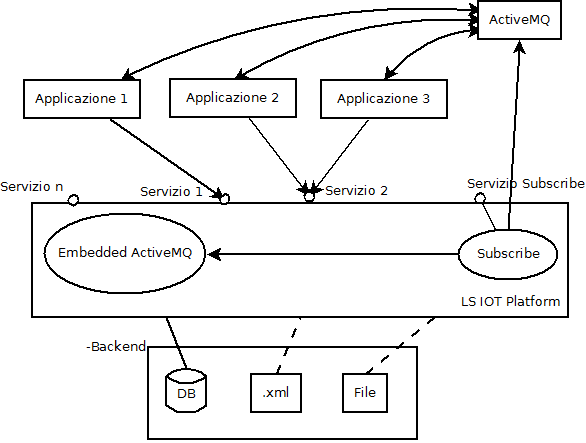
\includegraphics[width=0.8\textwidth]{architettura-piattaforma.png}
	\caption*{Figura 1. Schema della LS IOT Platform}
\end{figure}
La parte principale della piattaforma è il web server con i servizi REST. I servizi della piattaforma interagiscono con diverse applicazioni che inviano richieste HTTP per ottenere dati. Le applicazioni sono autenticate dalla piattaforma tramite un \textit{token} di abilitazione. Ciò che la piattaforma restituisce è rappresentato dalle sorgenti dati nel back end; nel nostro \textit{use-case} comprende un singolo database, ma può essere composto da più sorgenti eterogenee. Si aggiunge poi il servizio di "subscribe" che notifica le applicazioni sottoscritte tramite ActiveMQ (che può essere lanciato sia interno alla piattaforma che come servizio esterno).
Al momento i servizi sono legati all’interfacciamento con il database della Logical System s.r.l. nel quale sono riportate letture di sensori collegati a dei macchinari utensili. I valori dei sensori all'interno del database sono identificati tramite un codice che rappresenta il canale di ingresso dei vari input del controllore logico.
I servizi attualmente disponibili consentono di:
\begin{itemize}
	\item Prelevare la lista dei PLC con la relativa descrizione, se presente.
	\item Prelevare l’ultima misura di un sensore.
	\item Prelevare tutte le misurazioni salvate per un dato sensore (questo e i seguenti servizi hanno 2 implementazioni poiché interagiscono con 2 tabelle differenti, in quanto per gli estrusori è presente un’altra tabella a causa dei maggiori parametri da registrare): \begin{itemize}
		\item In base ad una data.
		\item Nell’arco di una settimana a partire dalla data inserita.
		\item Nell’arco di un mese dalla data inserita.
		\item Nell’arco di 2 date specificate.	
	\end{itemize}
	\item Prelevare le misure da una tabella tramite una sottoscrizione.
\end{itemize}
%\clearpage
La struttura dell’URL dei servizi viene elencata da questa tabella.
\begin{center}
	\begin{tabular}{ | l | p{5.06cm} | p{5.06cm} |}
		\hline
		\textbf{Servizio} & \textbf{Input} & \textbf{Output} \\ \hline
		getLastMeasure & \textit{ID} sensore / \textit{annotazione} & Ultima misura   \\ \hline
		getMeasureFromTo & \textit{ID} sensore / data \textit{Da} / data \textit{A} / \textit{annotazione} & Tutte le misure storicizzate da \textit{Data} a \textit{Data} \\ \hline
		getDetailedMeasureFromTo & \textit{ID} sensore / data \textit{Da} / data \textit{A} / \textit{annotazione} & Tutte le misure storicizzate prese dalla tabella degli estrusori / da \textit{Data} a \textit{Data} / \textit{annotazione}  \\ \hline
		getMeasureLastMonth & \textit{ID} sensore / Data (\textit{Today}) / \textit{annotazione} & Tutte le misure dalla data \textit{Today} a un mese prima \\ \hline
		getMeasureLastWeek & \textit{ID} sensore / Data (\textit{Today}) / \textit{annotazione} & Tutte le misure dalla data \textit{Today} a una settimana prima \\ \hline
		getDetailedMeasureLastMonth & \textit{ID} sensore, Data (\textit{Today}) / \textit{annotazione} & Tutte le misure dalla data \textit{Today} a un mese prima, degli estrusori \\ \hline
		getDetailedMeasureLastWeek & \textit{ID} sensore, Data (\textit{Today}) / \textit{annotazione} & Tutte le misure dalla data \textit{Today} a una settimana prima, degli estrusori \\ \hline
		subscribe & \{\textit{nome applicazione}, \textit{IP applicazione}, \textit{regola},\textit{coda o topic}\} & Misure del sensore caricate come messaggi sulla coda \\ \hline
		unsubscribe & \textit{ID regola} & Annullamento del servizio di subscribe \\ \hline
		getAllPlc & & Lista di tutti i sensori che la piattaforma offre con la relativa descrizione \\ \hline
	\end{tabular}
\end{center}
L'annotazione è un flag che indica se si vogliono ottenere i dati correlati dalla loro ontologia: inviare una richiesta con questo flag a false, restituisce i dati senza la loro ontologia. \capitalgrave{E} stata inserita nell'URL dei servizi perché presente nella lista degli sviluppi futuri previsti per la piattaforma, in modo da avere un punto di partenza per la sua completa implementazione.
\clearpage
\subsection{Database Use Case Aziendale}
Il database con le misurazioni dei sensori è costituito da sette tabelle. Tre tabelle contengono i valori letti ed elaborati dai controllori logici legati a sensori collegati ai vari macchinari in produzione che ripetutamente restituiscono questi valori; le altre quattro tabelle, se unite con una query, conterranno informazioni riguardo l’ontologia delle misure e delle misurazioni. La struttura dei record nelle tre tabelle dei dati è la stessa per tutti i macchinari, ma l’interpretazione dei valori cambia in base alla tipologia del macchinario e alla famiglia di appartenenza.
\begin{figure}[H]
	\centering
	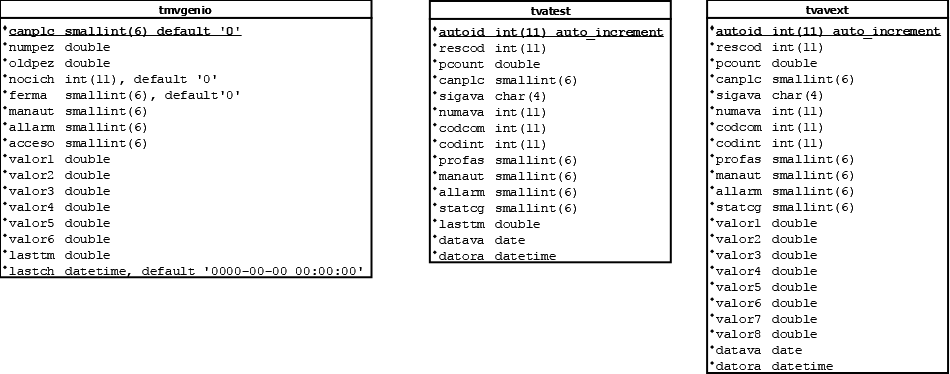
\includegraphics[width=0.8\textwidth]{tabelle-backend.png}
	\caption*{Figura 2.  Struttura delle tre tabelle dei dati}
\end{figure}
Tutte le informazioni relative all’ultima lettura di un sensore vanno nella tabella principale \textit{tvmgenio}. I dati che il controllore logico rileva sono inseriti in maniera diretta su un singolo record all’interno di questa tabella; quindi per ogni lettura viene creata una nuova riga contraddistinta dal canale di input al quale sono arrivati i dati. 

Le tabelle \textit{tvavtest} e \textit{tvavext} sono utilizzate per la storicizzazione dei dati. La prima per la storicizzazione generica di tutte le misurazioni, l’altra per la storicizzazione delle misurazioni dei macchinari estrusori. Per il fatto che contiene molti più valori parametrici aggiuntivi rispetto alla precedente tabella, è stata anche definita come dettagliata (i servizi riferiti a questa tabella contengono la parola “detailed”).


Una famiglia di un sensore specifica cosa rappresentano i valori e le misurazioni che sono effettuate. Quindi ad una famiglia sarà associata una ontologia delle misure e delle misurazioni. Riferita a questa ontologia si ha un servizio apposito che viene utilizzato per presentare il catalogo di sensori offerti dalla piattaforma. Ogni sensore ha la sua lista di campi con la loro ontologia e descrizione. In questo modo chi si registra nella piattaforma, è in grado di informarsi per quali sensori inviare richieste ai servizi REST. Il catalogo dei controllori logici è consultabile sia da applicazioni, il quanto il servizio restituisce un JSON contenente tutte queste informazioni, e da utenti: è presente anche una pagina web che converte questo JSON in una tabella.

Tutti i record delle tre tabelle dei dati hanno un campo che rappresenta il contatore principale dell’azione svolta dal macchinario. Questa informazione cambia di significato da un macchinario all’altro. Infatti per i sensori collegati a dei silos, il contatore principale rappresenta la quantità di materiale presente in chili, mentre per gli estrusori rappresenta i metri di tubo prodotti.
\clearpage
\subsection{Use Case Diagram}
\begin{figure}[h]
	\centering
	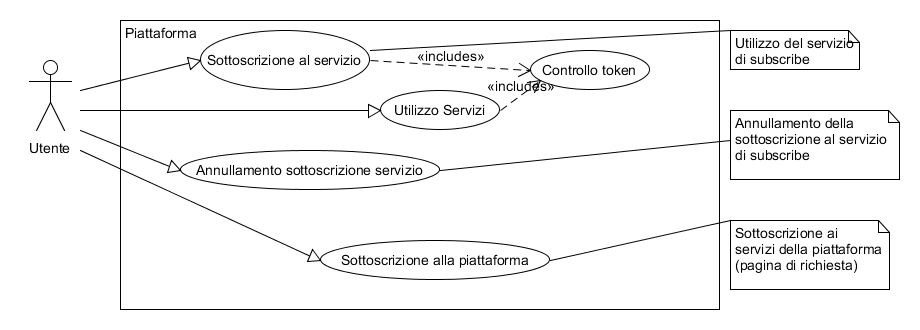
\includegraphics[width=0.8\textwidth]{use-case-utente.png}
	\caption*{Figura 3. Use case lato utente}
\end{figure}
Lo use case lato utente mostra le operazioni che l’utente è in grado di fare nella piattaforma. L’utente può usare i servizi della piattaforma, questa operazione include il controllo del token perchè per poter usare i servizi l’utente deve essere riconosciuto come abilitato. Può usare il servizio di subscribe (sempre se abilitato): questo speciale servizio permette di essere notificati tramite metodologia push riguardo i dati della piattaforma, seguendo largamente il modello publisher/subscriber: appena si verifica la condizione specificata, il servizio informa l’utente inviando il cambiamento dei dati. In altre parole, realizza un servizio di monitoraggio dati per l’utente. La sottoscrizione a questo servizio può essere annullata in qualsiasi momento tramite il servizio unsubscribe. Il token viene richiesto in una apposita pagina web e la sottoscrizione alla piattaforma viene gestita dall’amministratore.

\begin{figure}[h]
	\centering
	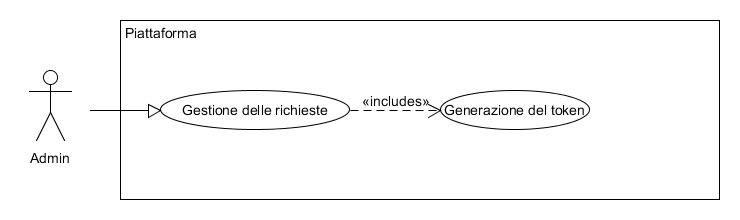
\includegraphics[width=0.8\textwidth]{use-case-admin.png}
	\caption*{Figura 4. Use case lato amministratore}
\end{figure}

Infatti come si vede dallo use case per l’amministratore, è lui che effettua la generazione del token a fronte di una richiesta di sottoscrizione alla piattaforma. Una richiesta può anche essere rifiutata.
\clearpage
\subsection{Class Diagram}
Il class diagram risulta essere troppo grande per essere comprensibile all’interno di una singola immagine, perciò ne verranno descritti alcuni frammenti. \par
\begin{figure}[h]
	\centering
	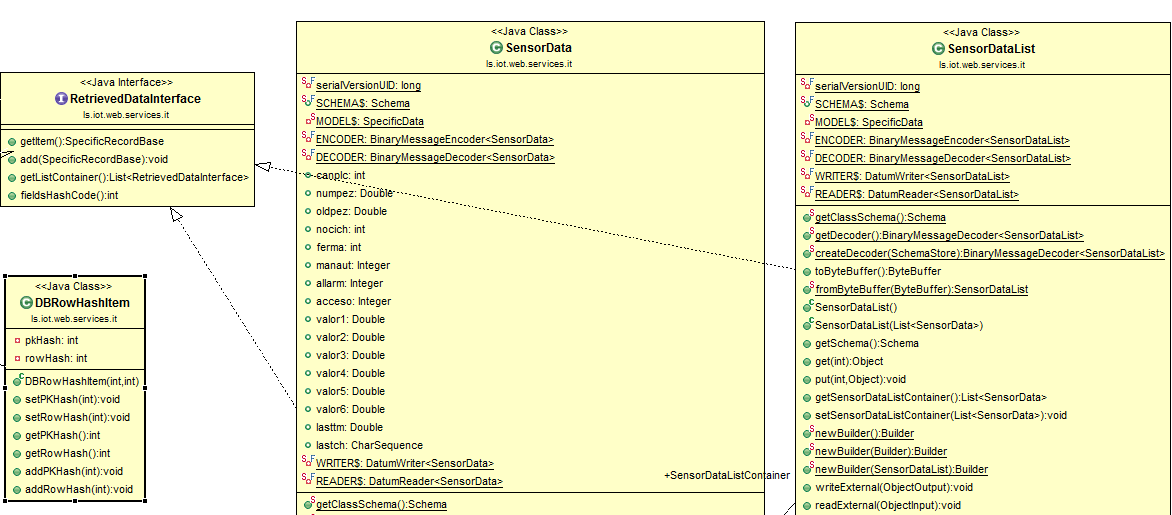
\includegraphics[width=0.8\textwidth]{sensor-data.png}
	\caption*{Figura 5. SensorData e SensorDataList con interfaccia}
\end{figure}
In figura 5 è descritta la classe SensorData che si ottiene compilando lo schema avro. I nomi delle proprietà della classe hanno lo stesso nome dei campi della tabella in modo da avere una relazione univoca tra proprietà dell’oggetto e campo del record del database. In questo modo è possibile assegnare valori all’oggetto Avro con la chiamata di un solo metodo. SensorDataList è l’oggetto Avro che rappresenta il contenitore (quindi l’array JSON) di questi oggetti. Si vede infatti la proprietà sensorDataListContainer che è legata da una relazione 0..* con la classe SensorData: un sensorDataListContainer può contenere zero o più oggetti SensorData. Per come è stata implementata la piattaforma ogni oggetto Avro deve avere il rispettivo oggetto contenitore nello schema. L’interfaccia RetrievedDataInterface rappresenta i metodi che ogni oggetto che si vuole restituire da un servizio REST, deve implementare. I metodi sono getItem per ottenere l’oggetto effettivo, getListContainer e add per ottenere l’oggetto contenitore nel caso in cui l’oggetto effettivo è una lista e per aggiungere un nuovo oggetto alla lista; i metodi per gli oggetti contenitore sono nella stessa interfaccia perchè salendo nella gerarchia delle classi degli oggetti Java generati con Avro, non c’è distinzione tra un oggetto contenitore e un oggetto singolo, entrambi ereditano dalla stessa classe SpecificRecordBase. Semplicemente un oggetto singolo restituirà \textbf{null} come listContainer e non eseguirà nessuna azione per l'inserimento. il metodo fieldsHashCode è necessario per ottenere l’hashcode dell’oggetto usando solo i valori delle proprietà: serve per definire se due oggetti sono identici considerando le proprietà dell'oggetto definite nel metodo. Usando RetrievedDataInterface è possibile interagire con qualsiasi sorgente dati nella backend purchè venga definito un oggetto Avro che rappresenti i dati che contiene. In questo modo la piattaforma può evolvere e gestire diversi schemi Avro di differenti oggetti.
\clearpage
\begin{figure}[h]
	\centering
	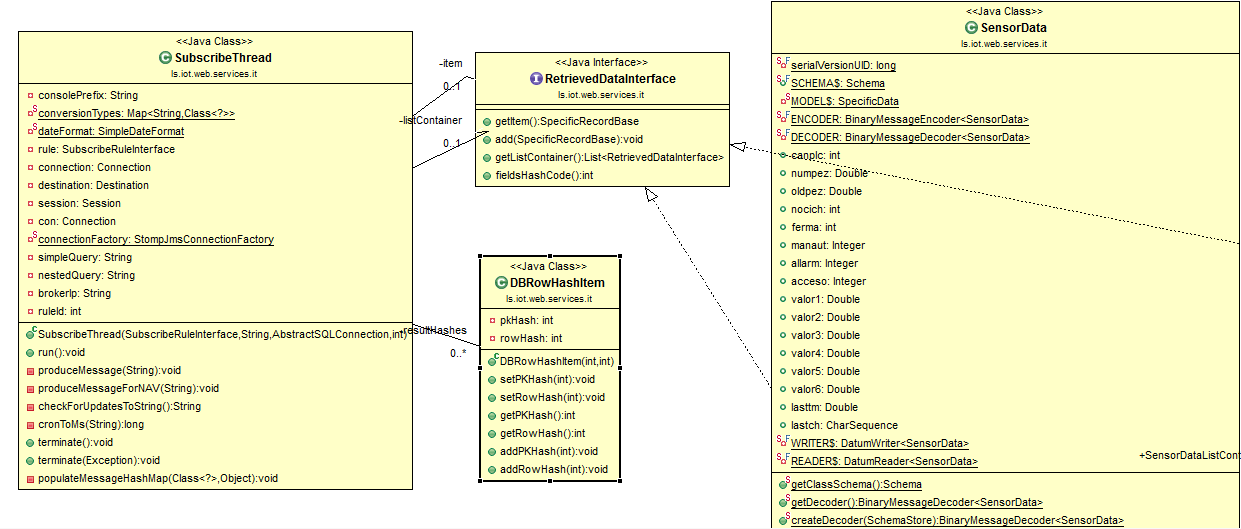
\includegraphics[width=0.8\textwidth]{subscribe-thread.png}
	\caption*{Figura 6. SubscribeRule e SubscribeThread con interfaccia}
\end{figure}
In figura 6 è rappresentato l’oggetto \textit{thread} che viene mandato in esecuzione quando un'applicazione effettua una sottoscrizione al servizio subscribe della piattaforma. Il thread contiene tutte le informazioni necessarie per eseguire query alla sorgente dati (rappresentata dall’oggetto connessione) che sono: la regola che deve eseguire ad ogni intervallo di tempo (intervallo CRON) e riferimenti al broker di messaggistica dove andrà a scrivere i nuovi dati che sono cambiati.
Una regola rappresenta un insieme di informazioni relative ad una specifica tabella nel backend che dichiarano la query di interrogazione da eseguire.
\par \vspace*{2em}
\begin{figure}[h]
	\centering
	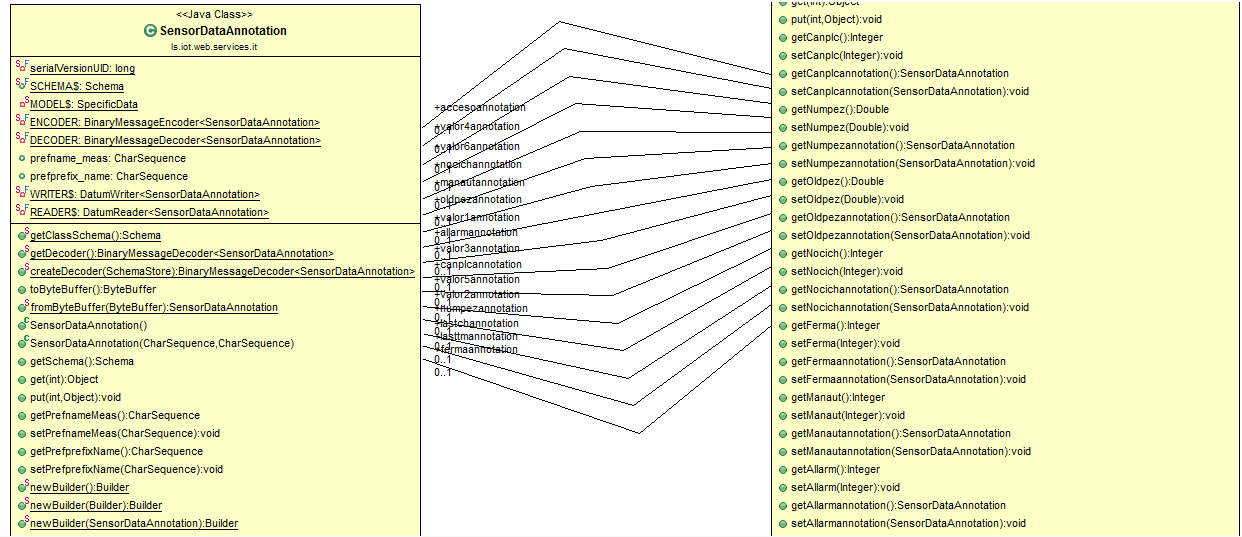
\includegraphics[width=0.8\textwidth]{sensor-data-annotation.png}
	\caption*{Figura 7. SensorDataAnnotation}
\end{figure}
In figura 7 è rappresentato l’oggetto annotazione che è presente negli oggetti Avro del caso d’uso aziendale. L’annotazione rappresenta l’ontologia legata alla misura (e non alla misurazione) che ogni singola proprietà dell’oggetto rappresenta. I campi che costituiscono una annotazione sono il nome dell’ontologia di riferimento e il suo ID.
\clearpage
\begin{figure}[h]
	\centering
	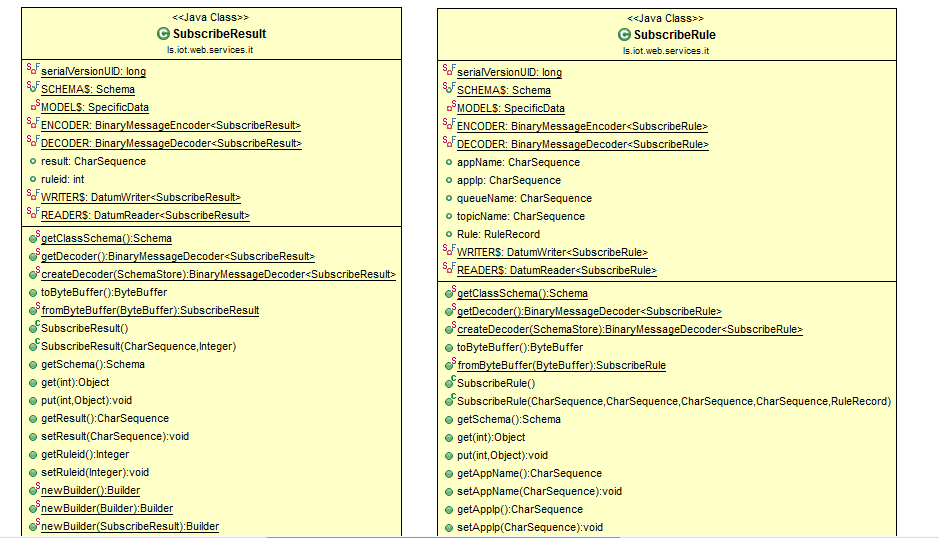
\includegraphics[width=0.8\textwidth]{subscribe-result.png}
	\caption*{Figura 8. SubscribeRule e SubscribeResult}
\end{figure}
In figura 8 è rappresentato l'oggetto ricavato dallo schema Avro che rappresenta l'oggetto contenente la regola di sottoscrizione che è utilizzato dalla piattaforma. La seconda classe rappresenta l’oggetto che viene restituito ad una applicazione ad indicare l’esito della sottoscrizione al servizio di subscribe. L’oggetto SubscribeRule ha come proprietà il nome dell’applicazione, l’ip dell’applicazione, la coda o topic di ActiveMQ in cui dovrà andare a scrivere e la regola che definisce la query SQL. L’oggetto SubscribeResult ha come proprietà semplicemente un messaggio result e un valore intero che rappresenta l’ID che il server ha associato alla regola cui riferisce. Questo identificativo viene usato nel caso in cui l’utente vuole annullare la sottoscrizione al servizio di subscribe.
\par \vspace*{2em}
\begin{figure}[h]
	\centering
	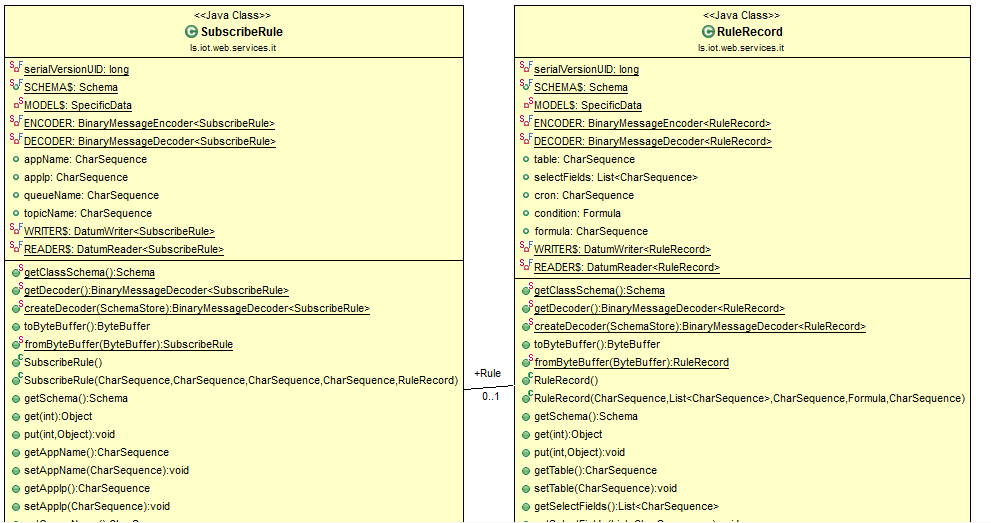
\includegraphics[width=0.8\textwidth]{rule-record.png}
	\caption*{Figura 9. SubscribeRule e RuleRecord}
\end{figure}
In figura 9 viene visualizzato più nel dettaglio l'oggetto RuleRecord, che definisce la query SQL di un SubscribeResult.
Un oggetto RuleRecord contiene: l’array dei campi del database dei quali si vuole essere notificati (l’utente viene notificato solo se viene registrato un cambiamento per questi campi); la tabella da interrogare; il CRON in formato stringa e la clausola where che è rappresentata da condition e formula. Condition rappresenta la definizione della where in maniera complessa, formata da più oggetti annidati; mentre formula rappresenta la where in una semplice stringa scritta a mano. 
\par \vspace*{2em}
\begin{figure}[h]
	\centering
	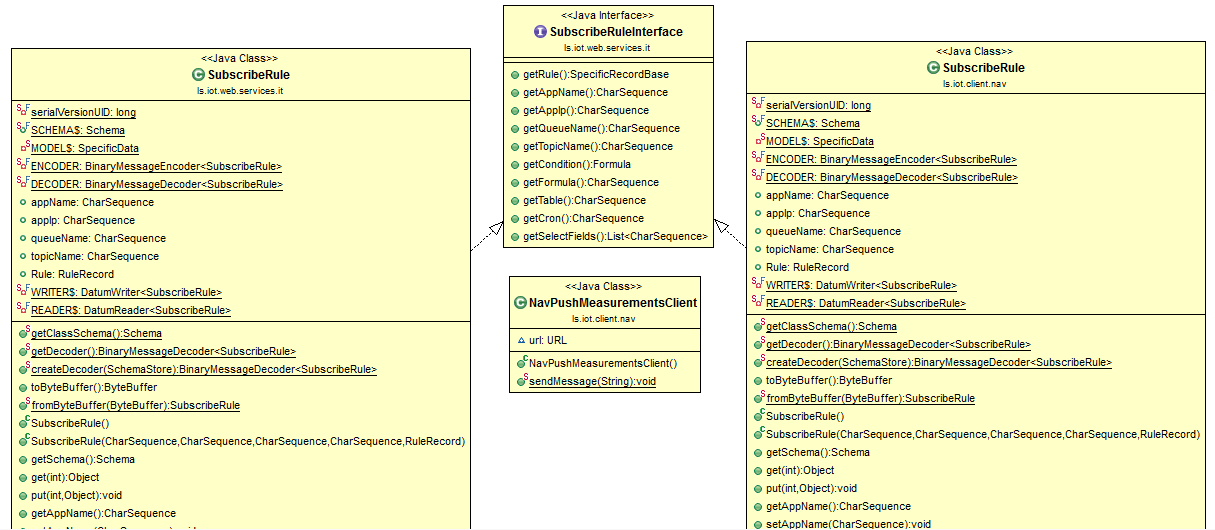
\includegraphics[width=0.8\textwidth]{rules.png}
	\caption*{Figura 10. SubscribeRule generale e per NAV con interfaccia}
\end{figure}
Per rendere la regola generica e implementabile in ogni situazione è  definita un’interfaccia, come descritto in figura 10. Questa interfaccia implementa i metodi necessari per rappresentare una regola, quindi metodi che restituiscono i campi della query, la tabella, la where e il CRON.

Il problema che ha fatto nascere il bisogno di questa interfaccia è il seguente. La piattaforma utilizza lo schema della regola complesso in cui la query SQL può essere definita come formula o come condition, e condition è un valore opzionale. Anche se condition è opzionale, quindi può non essere presente nel JSON che arriva al servizio di subscribe, nell’atto pratico deve esserlo con il valore di default\footnote{https://stackoverflow.com/questions/22939391/generating-an-avro-schema-with-optional-values}. Microsoft Dynamics NAV usa uno schema diverso da quello della piattaforma, una versione semplificata della regola in cui la condition non è definita perché in Microsoft Dynamics NAV non si può creare una finestra di input in cui ogni operazione viene aggiunta in maniera incrementale, perciò la query viene indicata direttamente come stringa. Questo significa che se la piattaforma implementa lo schema complesso della regola, quando riceve richieste di subscribe da parte di un client Navision, non è in grado di processare la richiesta in quanto nello schema non è presente il valore condition. Mentre se si fa in modo che la piattaforma accetti regole di tipo SubscribeRuleInterface, riesce a gestire regole sia di Navision che di altre applicazioni.
\clearpage
\begin{figure}[h]
	\centering
	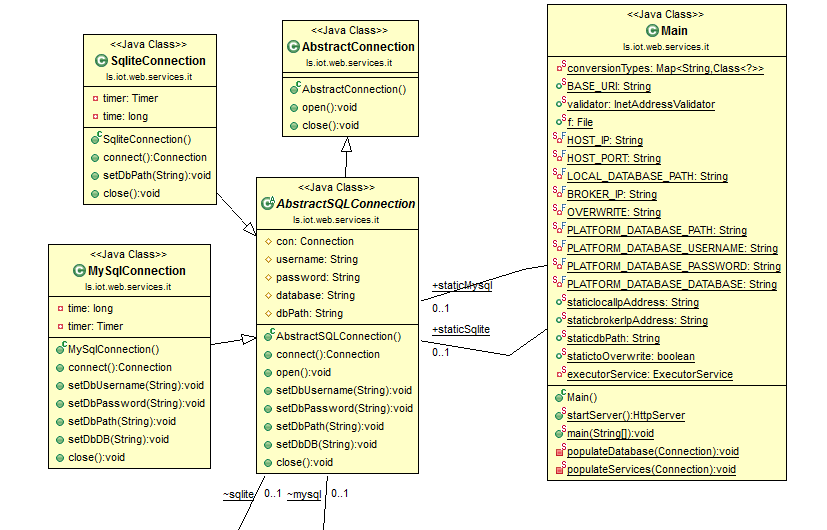
\includegraphics[width=0.8\textwidth]{main.png}
	\caption*{Figura 11. Classe astratta per gestire le connessioni}
\end{figure}

La figura 11 rappresenta la gestione delle connessioni nella piattaforma. Per poter estendere la backend a qualsiasi sorgente dati, è stata definita una classe astratta AbstractConnection che ha come metodi generali open e close, di primaria funzione per ogni sorgente come file o database. Questi metodi possono essere quindi sovrascritti in base al corretto funzionamento desiderato, da classi che rappresenteranno l’implementazione concreta della connessione. Per il nostro use case è necessario inoltre avere connessioni a database SQL perciò è stata definita la classe astratta AbstractSQLConnection che rappresenta una connessione qualunque ad un database SQL: ha come proprietà il path in cui si trova il database,  username e password per collegarsi e il nome del database. Questa classe così definita rappresenta connessioni sia a database MySQL, dove solitamente ci si collega ad un server, sia connessioni di tipo SQLite dove il database è un file su disco. Le implementazioni fisiche sono quindi differenziate per MySQL e Sqlite a cui sono state aggiunte un timer per fare in modo di chiudere la connessione dopo 10 minuti di inutilizzo.
\clearpage
\section{Struttura Dati Json}
L’utilizzo del framework Avro ha questi vantaggi\footnote{http://blog.cloudera.com/blog/2011/05/three-reasons-why-apache-avro-data-serialization-is-a-good-choice-for-openrtb/}:
\begin{itemize}
	\item Avro può gestire in maniera dinamica i dati, utile in situazioni dove lo schema dei file non è noto al momento della compilazione. La gestione dinamica non richiede di generare una classe da utilizzare all’interno del programma, ma avviene tramite un GenericRecord. In questo modo i dati possono essere inseriti con dei metodi put.
	\item Mentre nella gestione dei dati con l’utilizzo di classi che contengono lo schema (code-generation)\footnote{https://stackoverflow.com/questions/30277442/what-does-code-generation-mean-in-avro-hadoop}, i metodi get/put che permettono di accedere ai dati sono auto esplicativi ed esiste un metodo per ogni campo definito nello schema. Inoltre i metodi di get e put accettano come parametro anche il nome del campo e quindi il vantaggio dell’utilizzo di Avro si vede, ad esempio, nella popolazione dell’oggetto SensorData. 	
\end{itemize}
La struttura che abbiamo definito per rappresentare i dati della tabella \textit{tvmgenio} è la seguente.
{\fontfamily{pcr}\selectfont
\lstinputlisting[breaklines]{sensor-data.txt}
}

Vengono ripresi gli stessi nomi dei campi del record, in modo da avere una relazione diretta e inserire quindi i valori tramite il metodo put.

Inoltre sono presenti i campi delle annotazioni, che sono altri oggetti contenenti i valori di ID e nome dell’ontologia della misura. L’ontologia delle misure nello schema Avro è chiamata annotazione ed è un valore opzionale.
L’annotazione cambia il comportamento dei servizi della piattaforma, infatti se viene richiesta, la query di interrogazione dei dati e il popolamento della lista contenitore cambiano. Per come è strutturato il database aziendale, quando l’annotazione viene richiesta, lo stesso oggetto della tabella viene ripetuto più volte, per ogni annotazione che ha, e per evitare di trasferire tutto il ResultSet in una variabile in memoria, come un HashSet, per evitare ripetizioni degli stessi risultati, si è scelto di fare tutto mentre si scorre l'insieme di record, tenendo conto del valore precedente dell’oggetto: nel caso in cui l’oggetto è lo stesso, i campi vengono saltati e si passa a popolare solo l’oggetto annotazione che non viene inserito all’interno del nuovo oggetto ma in quello precedente. In questo modo si ha sempre una sola versione dello stesso oggetto con le annotazioni aggiornate. Per questa modalità di inserimento e gestione si è dovuto fare un controllo aggiuntivo sul fatto di essere arrivati all’ultima riga del ResultSet, perché inserendo il valore precedente quando non corrisponde al valore attual avviene che, arrivati all’ultimo elemento questo non verrà mai inserito.

Gli schemi Avro per le altre tabelle per la storicizzazione, rispettivamente SensorHistoricalData per tvavtest e SensorHistoricalDataExt per tvavext, sono fatte allo stesso modo di SensorData.
%\clearpage
\subsection{Struttura della regola di subscribe}
Lo schema Json che rappresenta una regola per il servizio di Subscribe è il seguente. 
{\fontfamily{pcr}\selectfont
	\lstinputlisting[breaklines]{subscribe-rule.txt}
}
Nel messaggio JSON che il servizio di subscribe riceve viene specificato, il nome e l’indirizzo IP dell’applicativo che richiede la sottoscrizione, il nome della coda o del topic del message broker e la regola, un oggetto chiamato SubscribeRule che contiene tutte le informazioni riguardo la query SQL che indica a quali dati chi richiede il servizio è interessato.
\clearpage

\subsection{Struttura della Condition}
Nell'oggetto \textit{condition} le operazioni SQL sono descritte da enum che hanno come simboli tutti i possibili operatori. Sono presenti:
\begin{itemize}
	\item operatori di confronto
	\item operatori aritmetici
	\item operatori per le operazioni bit a bit
	\item operatori binari
	\item operatori che si applicano ad altre sub-query come ANY, ALL e SOME
\end{itemize}
Il punto di partenza di una \textit{condition} è un oggetto Formula che può essere espresso in un oggetto FormulaOperation. Da questo oggetto FormulaOperation si differenziano operazioni che comprendono gli operatori sopra descritti.

Uno schema che rappresenta l'evoluzione di un oggetto Condition è rappresentato in figura 13.
\begin{figure}[h]
	\centering
	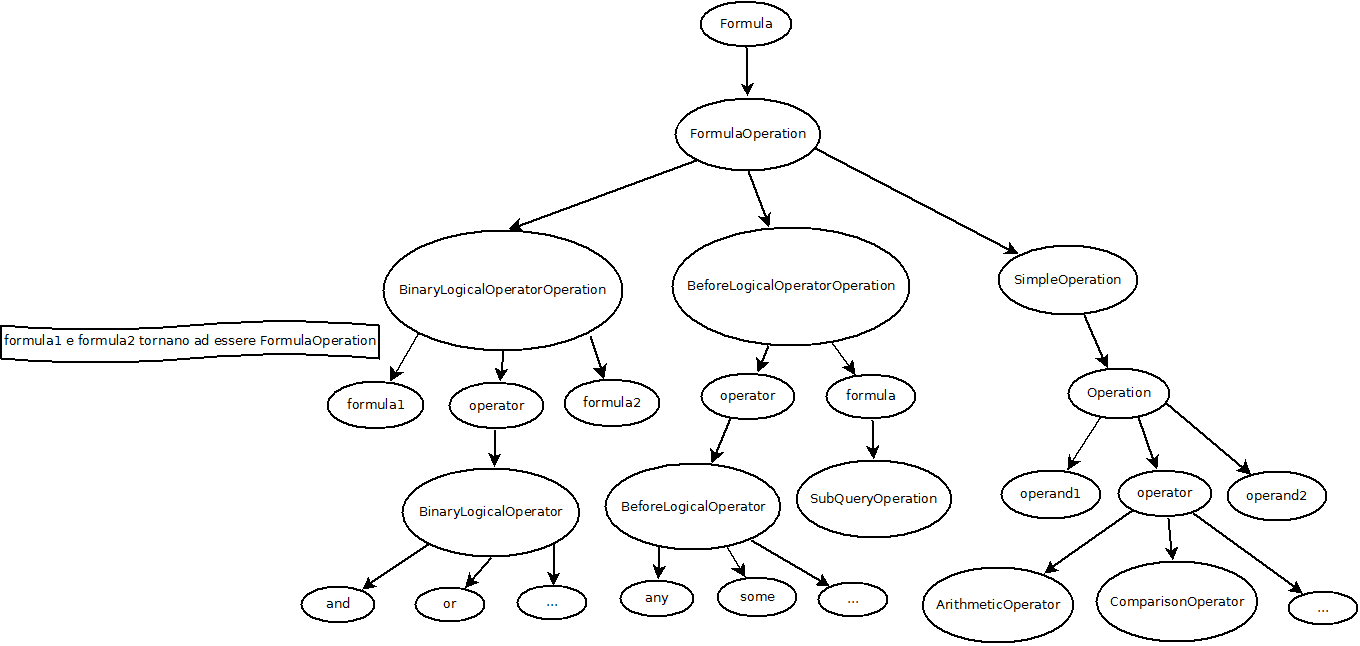
\includegraphics[width=0.8\textwidth]{struttura-query-tree.png}
	\caption*{Figura 13. Schema ad albero della definizione di condition}
\end{figure}
\clearpage
Un generico JSON che potrebbe essere inviato al servizio di Subscribe da parte di un applicazione è rappresentato in figura 12.
\begin{figure}[H]
	\centering
	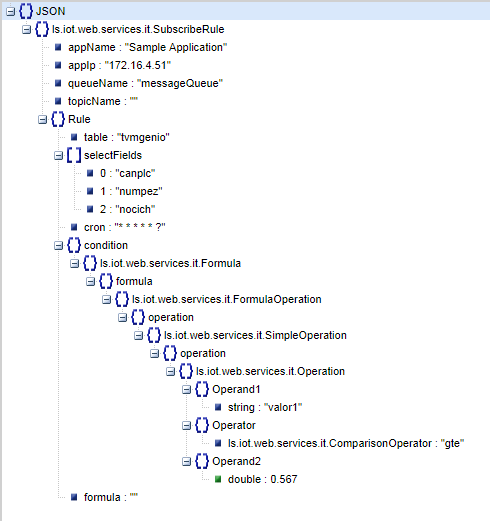
\includegraphics[width=0.4\textwidth]{subscribe-json-1.png}
	\caption*{Figura 12. SubscribeRule in formato Json}
\end{figure}

Mentre lo schema Avro della SubscribeRule inviata da parte di un client Microsoft Dynamics NAV viene descritto da questo schema.
\begin{center}
		{\fontfamily{pcr}\selectfont
			\lstinputlisting[breaklines]{subscribe-rule-nav.txt}
		}
\end{center}
A differenza dello schema principale, in questo schema la query SQL può essere definita solo come stringa. 

In figura 14 è descritto un possibile JSON che potrebbe essere inviato al servizio di subscribe da parte di un client Navision.
\begin{figure}[h]
	\centering
	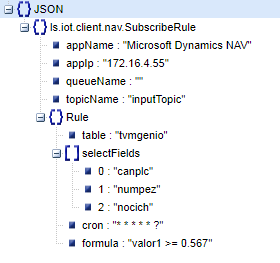
\includegraphics[width=0.4\textwidth]{subscribe-json-2.png}
	\caption*{Figura 14. SubscribeRule in formato Json proveniente da NAV}
\end{figure}

Viene usato Avro anche per la regola di Subscribe per avere una soluzione robusta e sicura, e avere un controllo immediato per evitare di ricevere JSON malformati. Nel momento in cui il JSON arriva al server, è in formato stringa senza nessun controllo; viene poi convertito in un byte array, il formato serializzato che Avro può interpretare, seguendo proprio uno schema. In questo modo si riesce poi a istanziare un oggetto che rappresenta una regola di subscribe, per le operazioni come la creazione del thread, o la creazione della coda nel broker di messaggistica, si prendono i dati direttamente dall'oggetto anziché effettuare il parsing in base al nome dei campi dalla stringa JSON.

\section{Servizio di Subscribe}
Il servizio di subscribe è composto da un oggetto Executor che organizza un “pool” di thread, di numero indefinito. L'esecuzione di questi thread viene gestita dall’executor stesso. Un thread rappresenta l’oggetto che ha il compito di gestire una singola regola ricevuta dal servizio. La gestione dei thread rimane possibile grazie al metodo submit dell executor che restituisce un Future$\langle?\rangle{}$. Questo tipo di oggetto rappresenta lo stato di esecuzione di un thread e grazie a questo è possibile fermarlo in qualsiasi momento chiamando il metodo terminate. Il servizio di Subscribe, per tenere traccia di ogni thread che è stato creato, gestisce una hashmap che associa all’id della regola ricevuta dal servizio il thread che andrà a gestirla. 

Il server una volta che riesce a mandare in esecuzione correttamente un thread, restituisce un JSON che indica se l’operazione è andata a buon fine. Lo schema di questo oggetto SubscribeResult è il seguente.
\begin{center}
		{\fontfamily{pcr}\selectfont
			\lstinputlisting[breaklines]{subscribe-result.txt}
		}
\end{center}
Questo oggetto definisce un messaggio result che indica il termine dell’operazione e un valore numerico che rappresenta l’ID associato alla regola che l'applicazione potrà poi usare per annullare la sottoscrizione a questo servizio.
Il thread per capire se i dati sono cambiati nel database, mantiene una struttura dati che contiene l’hashcode dei record che ottiene dalla query. Questo hashcode è salvato in un oggetto che, in due proprietà diverse, rappresenta l’hash della chiave del record e l’hash del corpo del record. Questa gestione permette di fare in modo che la posizione del valore hash nella hashmap non sia legato alla posizione del record nel ResultSet. In questo modo se il contenuto di un record cambia, indipendentemente dalla sua posizione, viene aggiornato nella hashmap seguendo i valori di chiave primaria (che sono fissi e non cambiano per definizione).

Il servizio di Subscribe notifica l'applicazione del cambiamento dei dati tramite un broker che funge da intermediario tra l'applicazione e la piattaforma. Per i client Microsoft Dynamics NAV non è stato possibile utilizzare lo stesso sistema di una coda ActiveMQ, per la mancanza di NAV di poter avere un servizio sempre attivo che andasse a leggere nella coda. Per questo Navision ha un servizio ad hoc nel quale il thread che gestisce la sua sottoscrizione va scrivere i dati dei quali ha notato un cambiamento e NAV aggiungerà questi nuovi dati in una tabella. Il client Java per inviare messaggi al servizio di NAV è stato generato automaticamente tramite la WSDL messa a disposizione proprio dal servizio di NAV. Inoltre nel connettersi al servizio, bisogna autenticare il client Java con un profilo che abbia i permessi di scrivere nel servizio NAV. L’autenticazione avviene tramite il profilo dell'utente Windows con il protocollo NTLM.

\section{Token Authentication}
Un client per poter utilizzare un servizio deve essere abilitato. L'abilitazione ai servizi della piattaforma si ottiene tramite una apposita pagina. Nella pagina di richiesta le informazioni da inserire sono il nome dell’applicazione, il suo IP, le credenziali che si vorranno usare per accedere alla pagina personale di gestione dei servizi e un indirizzo email, tramite il quale l'utente che effettua la richiesta di abilitazione  verrà notificato del suo token. Una volta inviata una richiesta, questa viene inserita all’interno del database di amministrazione, che con una tabella chiamata Requests riferisce tutte le richieste di token che sono state ricevute. Il token è una stringa di caratteri alfanumerici che rappresenta l’abilitazione dell’utente all’utilizzo dei servizi della piattaforma. È generato tramite la classe UUID di java in modo da garantire l’univocità di ogni token.

Una pagina di gestione permette ad un amministratore di abilitare una applicazione ad usare i servizi, quindi genererà un token specifico per quell'applicazione.
Una volta ottenuto il token, l’utente che si è sottoscritto ad usare i servizi deve impostarlo nell’header di ogni richiesta. Un'altra tabella nello stesso database amministrativo contiene tutti i token che sono stati rilasciati alle applicazioni. Se un token che arriva ad un servizio rientra nei token registrati, allora chi vuole usare quel servizio può farlo.

Con il sistema del token è stato implementato anche un sistema per tenere traccia delle statistiche di utilizzo dei servizi da parte delle applicazioni. Nel database amministrativo è presente una tabella dei servizi contenente nome e ID di tutti i servizi che sono presenti nella piattaforma. Avendo associato un ID ad ogni servizio, è possibile tenere delle variabili per ogni ID: quando un utente effettua una richiesta di abilitazione, sceglie quali servizi vuole attivare e in questo modo popola una lista che contiene l’ID di ogni servizio che vuole gli sia abilitato. Quando la richiesta viene accettata, questa lista è inserita nella tabella delle sottoscrizioni attive e ne viene generata una simile con tutti i valori a zero. Questa altra lista rappresenta l’utilizzo dei servizi, dove la posizione di un ID è la stessa nella lista degli utilizzi. In questo modo quando un utente che ha una lista di servizi attivi come questa [1,2,3] effettua una chiamata al servizio 3, nella lista degli utilizzi, il contatore nella terza posizione viene incrementato di 1 [0,0,1]. Questo avviene automaticamente durante il controllo del token.
\clearpage
\section{Gestione degli errori}
\subsection{Schema Avro}
\begin{center}
		{\fontfamily{pcr}\selectfont
			\lstinputlisting[breaklines]{exception-handler.txt}
		}
\end{center}

Per dare un feedback all’applicazione in caso di utilizzo errato dei servizi, viene restituito il messaggio di errore dell’eccezione che viene generata dal sistema come messaggio JSON, seguendo questo schema Avro. A questa eccezione è associato un numero che rappresenta l’hashcode della classe, in questo modo si definisce un codice di errore per categoria, ad esempio le eccezioni di tipo NullPointerException hanno il loro codice e IllegalArgumentException hanno il loro codice; e un livello di errore in base alla gravità di cosa è successo.

\section{Database Amministrativo}
La piattaforma ha come base di dati principale un database SQLite che contiene informazioni riguardo le richieste registrate; regole che sono attualmente attive; applicazioni abilitate ad usare la piattaforma e il loro utilizzo dei servizi.
In figura 15 è mostrata la gestione delle regole di subscribe attualmente attive.
\begin{figure}[h]
	\centering
	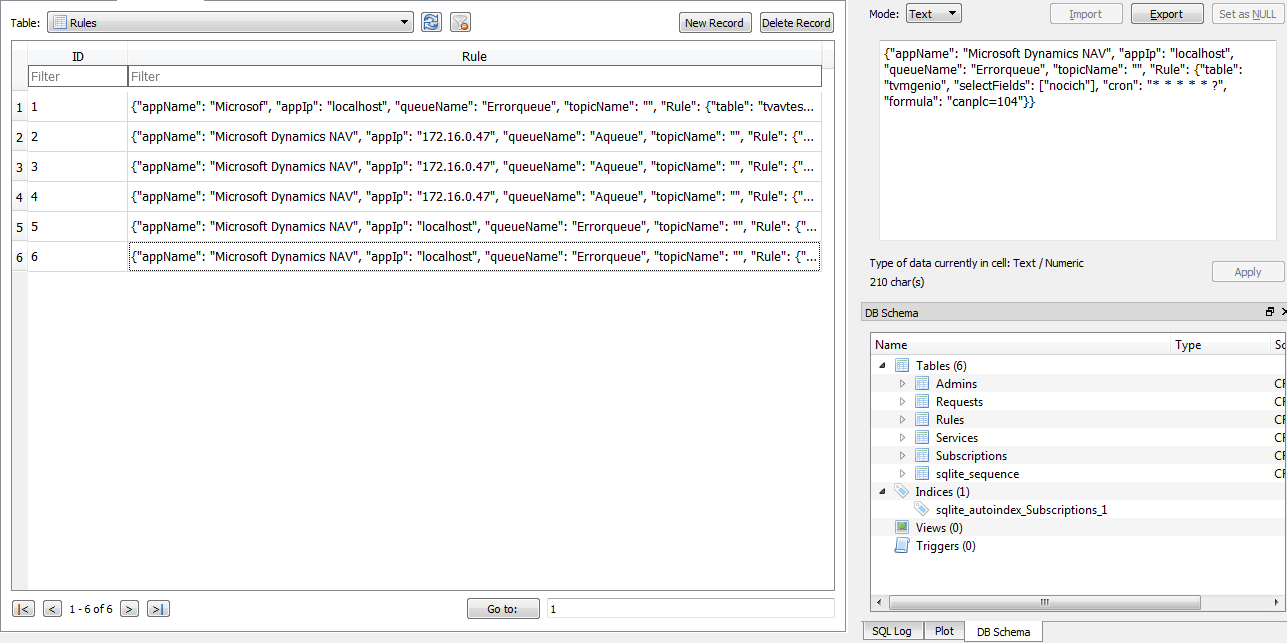
\includegraphics[width=0.8\textwidth]{db-rules.png}
	\caption*{Figura 15. Screenshot della gestione delle Rules}
\end{figure}
\clearpage
La piattaforma è in grado di creare il database amministrativo autonomamente, ad esempio nel caso in cui venga avviata per la prima volta, avendo codificate nel metodo principale, la struttura delle tabelle. In questo modo la piattaforma genera il suo ambiente di lavoro ogni volta che viene avviata in un nuovo contesto in cui il database non è presente. La piattaforma è così portabile e indipendente da dove viene lanciata, generando ogni volta il database con un amministratore di default.
La piattaforma ha anche questa funzionalità: per rispettare la struttura di un login in ambiente client/server, anche in assenza di un server php, una hashmap di sessioni regola il login degli utenti. Come session ID viene usato l’hashcode della stringa che si ottiene concatenando username e password dell'utente e la sessione contiene username e password di chi effettua il login in modo da poter inviare al browser un cookie contenente il session ID e permettergli di visualizzare il contenuto delle pagine. Il cookie ha durata di 1 ora e vale su tutto il dominio "/ls" della piattaforma.

\section{Espressioni CRON}
Le espressioni cron sono utilizzate in ambienti Unix-like per eseguire una determinata operazione in un determinato intervallo di tempo (per esempio ogni minuto 10 di ogni giorno). Utilizza una sintassi particolare formata nel modo seguente:
\begin{center}
	{\fontfamily{pcr}\selectfont
		\lstinputlisting[breaklines]{espressione-cron.txt}
	}
\end{center}
Dove l’anno è facoltativo. In cron è possibile inserire dei caratteri speciali come il ? (indicante nessun valore) e * (indicante ogni valore ammesso dall’intervallo).

\section{Architettura Lato Client}
Nell’architettura generale è previsto l’utilizzo di un client che è sempre attivo e rimane in attesa dell’embedded broker activemq che lo notifica con nuovi dati. Nel momento in cui questa applicazione viene interfacciata con Microsoft Dynamics NAV si hanno delle difficoltà in quanto non vi è la possibilità di ricevere dati in maniera push direttamente ma è necessario passare per un ulteriore step: l’utilizzo di un webservice SOAP da NAV\footnote{https://blogs.msdn.microsoft.com/freddyk/2010/01/19/connecting-to-nav-web-services-from-java/} con il quale è consentito esternare codeunit, pagine e query. In questo modo tramite il WSDL è possibile compilare automaticamente un client per quel webservice e interagire direttamente con quel servizio. Sarà così possibile la ricezione di dati sempre aggiornati successivamente alla sottoscrizione del servizio in base ad una regola specificata dall’utente senza dover necessariamente utilizzare tecniche di polling (con cui continuo a chiamare costantemente il server per sapere se vi sono nuovi dati).
\subsection{Breve Introduzione su Microsoft Dynamics NAV}
Microsoft Dynamics NAV è un software gestionale pubblicato da Microsoft. Esso consente alle imprese una completa gestione della contabilità e del magazzino tramite tabelle e pagine, dispone di un sistema centralizzato con autorizzazioni in modo che solo determinati utenti possano accedere a determinate aree di lavoro. NAV è suddiviso in client e ambiente di sviluppo (development environment) : nel client è possibile inserire e visualizzare dati, mentre nell’ambiente di sviluppo è possibile inserire codice C\textbackslash AL e costruire oggetti che poi verranno utilizzati nel client. Sia client che development environment lavorano su uno stesso servizio il quale deve essere disponibile su un server NAV. \newline
Gli oggetti costruibili nell’ambiente di sviluppo di Microsoft Dynamics NAV sono: 
\begin{itemize}
\item Tabelle (alla base, le quali contengono i dati che il client mostrerà).
\item Pagine (che consentono una vista sui dati di una o più tabelle).
\item Query (che consentono di effettuare operazioni di selezione sui dati delle tabelle).
\item Codeunit (classi in C\textbackslash AL code utilizzabili per compiere particolari operazioni sui dati).
\item XMLport (che consentono di importare file XML).
\item Report (che permettono di visualizzare e stampare dati dalle tabelle) .
\item Menusuite (i quali permettono di visualizzare un menu a lato nell’ambiente di sviluppo, per esempio per raggruppare gli oggetti necessari per un determinato sviluppo).
\end{itemize}
Oltre che nelle codeunit, all’interno di questi oggetti è inoltre possibile inserire del codice C\textbackslash AL in corrispondenza di determinati “trigger”, ovvero punti in cui un determinato evento è verificato. 
\section{Client C\#}
Per interagire con l’interfaccia LSIoT che fornisce servizi REST è necessario a sua volta avere un client in grado di consumare questi servizi. Nel nostro caso ci siamo occupati di interfacciare Microsoft Dynamics NAV con questa piattaforma sviluppata in Java ed è stato necessario estendere le funzioni del suo ambiente in quanto NAV non può direttamente utilizzare servizi REST. Con NAV è infatti possibile l’utilizzo di librerie realizzate in C\# e compilate come .dll. In questo modo è stato creato un client in grado di consumare servizi REST e utilizzarlo a sua volta all’interno dell’ambiente Navision, con successivo trattamento dei dati ricevuti.
\clearpage
\subsection{Class Diagram}
\begin{figure}[h]
	\centering
	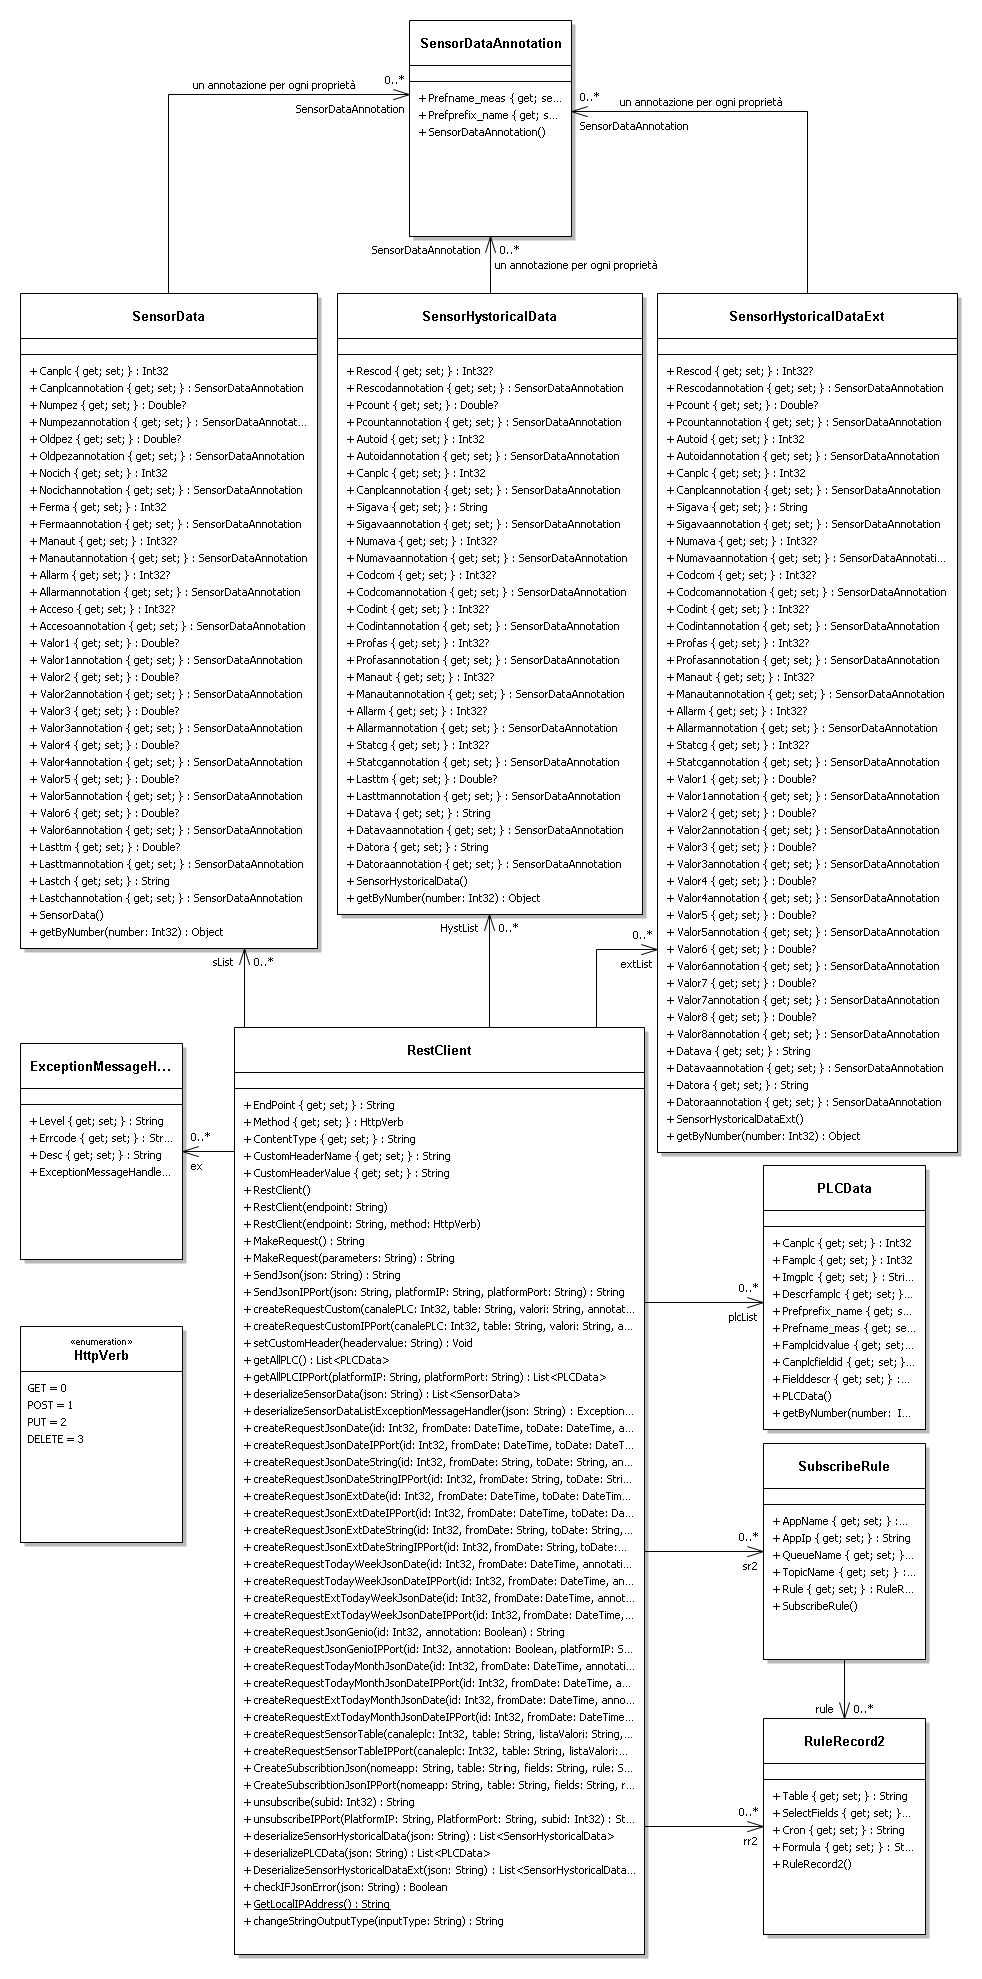
\includegraphics[width=0.47\textwidth]{class-diagram-client.png} \newline
	\caption*{Figura 16: Class Diagram Client C\#}
\end{figure}
\clearpage
Come si nota dal class diagram il client è composto da varie classi che sono utilizzate da un'unica classe RestClient, la quale si occupa di effettuare le vere chiamate ai servizi. Ogni metodo della classe RestClient relativo all’utilizzo dei servizi REST ha tra i parametri ciò che deve passare alla piattaforma tramite richiesta http in base al servizio, la connessione alla piattaforma e la deserializzazione della risposta. Inoltre ognuno di essi ha una seconda definizione che presenta tra i parametri anche la possibilità di inserire IP e porta della piattaforma. Questa scelta è stata fatta in quanto se si ci si vuole collegare ad un indirizzo diverso rispetto a quello impostato nei vari metodi (per esempio nel caso in cui la piattaforma cambi indirizzo IP) risulta possibile senza dover necessariamente cambiare il codice C\# e ricompilare dunque la dll. Per poter utilizzare questi servizi, è tuttavia necessario effettuare una sottoscrizione alla piattaforma. La sottoscrizione avviene tramite sito web e una volta iscritti viene assegnato un id della relativa sottoscrizione e, se la sua sottoscrizione è accettata, un token al richiedente che dovrà utilizzare quando chiama i vari servizi (dovrà essere inserito nell’header del messaggio http). Per quello che riguarda il servizio di subscription vengono anche inseriti altri dati oltre al nome del client richiedente e all’indirizzo come la coda su cui si vuole operare in activemq, ogni quanto tempo si vuole la ricezione dei dati aggiornati (tramite formula CRON), la condizione con la quale si vuole richiedere i dati (espressa praticamente come clausola where della chiamata SQL e la tabella dalla quale si andranno a ricevere i dati). In questo caso i dati verranno inviati al client a seconda delle condizioni stabilite dal subscription e, come per tutti i servizi vengono inviati in formato JSON.


Oltre ai metodi strettamente legati alla piattaforma vi sono anche metodi per prendere in maniera dinamica il proprio indirizzo IP e metodi di controllo del JSON, che potrebbe arrivare contenente semplicemente un errore con il tipo, codice e descrizione. Sia per l’errore che per il messaggio di sottoscrizione sono stati elaborati schemi avro e classi generate con i relativi metodi di deserializzazione. 

Le classi utilizzate da RestClient non sono state create a mano ma sono state generate automaticamente e formalmente dal software Apache Avro. 

Avro è utlizzato solitamente in ambiente java, ma è disponibile anche una versione per .NET, la quale tuttavia, genera delle classi con meno metodi rispetto alla controparte in Java, che nonostante ciò sono comunque molto utili per il loro scopo principale. Nonostante infatti non sia possibile nativamente generare il JSON direttamente da una classe generata da uno schema, queste classi rendono molto più semplice l’interazione con metodi e attributi di tali oggetti. Inoltre l’approccio formale garantisce che non vi siano differenze nei nomi degli attributi del JSON in quanto le classi sono generati dal medesimo schema.

Il client è stato utilizzato inizialmente come client REST C\# a se stante per testare l’utilizzo dei servizi forniti dalla piattaforma e successivamente è stato integrato, dopo aver generato la dll, nell’ambiente Navision. Il testing e la generazione della libreria avvengono sulla stessa soluzione ma in 2 progetti diversi, in modo da utilizzare i metodi dall’esterno, in maniera simile a quanto avviene su NAV.

Per quello che riguarda la connessione Il client REST usa il metodo MakeRequest dove si crea un istanza di WebRequest utilizzando l’indirizzo del servizio REST come URI (identificato come endpoint). Questa istanza viene convertita ad HttpWebRequest (in quanto chiamare HttpWebRequest.create corrisponde a chiamare create da WebRequest). Successivamente si imposta il metodo, la lunghezza e il tipo del contenuto e infine l’header http (necessario per passare il token utilizzato nella sottoscrizione ad un servizio). Si procede poi con la creazione dell’oggetto response, il quale conterrà la risposta (tramite chiamata del metodo request da getResponse,  si controlla che lo status code di risposta sia il 200 (ok) e si crea un oggetto Stream dal quale si andrà a leggere con uno streamreader ciò che è contenuto nel body della risposta (nel nostro caso il Json contente i risultati dal DB).
\clearpage
Per quello che riguarda l’invio di dati in formato JSON è stato creato un metodo con il quale si procede allo stesso modo del metodo MakeRequest ma stavolta si utilizzano 2 stream, uno streamwriter per mandare il mio JSON per la sottoscrizione al servizio “push” alla piattaforma e uno streamreader per ricevere la risposta della piattaforma contente un json con il risultato della sottoscrizione e l’id relativo.

Nonostante sia generalmente consigliato l’utilizzo di httpClient, è stato utilizzato HttpWebRequest\footnote{http://www.diogonunes.com/blog/webclient-vs-httpclient-vs-httpwebrequest/}. httpClient è più semplice e costruito sopra httpwebrequest per diminuire la quantità di codice da scrivere per effettuare una richiesta, ma non è compatibile con tutte le versioni del .NET Framework. Dato che il client NAV ha la possibilità di utilizzare metodi relativi alla versione 4.0 del .NET Framework per maggiore stabilità con NAV dunque si è adottata questa soluzione, ma in futuro non è escluso che si possa passare a all’utilizzo di httpclient.

Una volta che i dati in formato JSON arrivano correttamente al client C\# è dunque necessaria una deserializzazione dei dati tramite opportune classi corrispondenti al JSON di arrivo. Per la deserializzazione è stato utlizzato JSON.NET, un framework disponibile per ambiente .NET ed installabile tramite pacchetti NuGet. Questo framework consente di deserializzare e serializzare JSON con semplici e brevi istruzioni.


\begin{figure}[h]
	\centering
	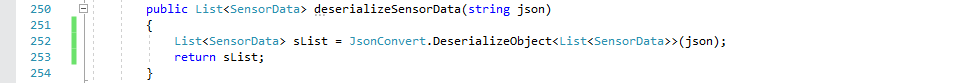
\includegraphics[width=0.8\textwidth]{deserialize.png}
	\caption*{Figura 17: Utilizzo del framework nella deserializzazione di un oggetto generato dallo schema avro.}
\end{figure}

Con questo framework è inoltre possibile la costruzione di JSON tramite codice con l’utilizzo di appositi metodi dell’oggetto JsonWriter (come ad esempio WriteStartObject, WritePropertyName, WriteValue ecc.). Proprio con questi metodi e con gli oggetti delle classi generati è stato possibile costruire il JSON per il servizio di subscribe.

In Microsoft Dynamics NAV si hanno 2 metodi per utilizzare le dll generate dagli utenti: mettendole sul client o sul server. Dato che, se una libreria è posizionata sul server, una sua modifica o sostituzione richiede un riavvio dell’intero servizio, inizialmente essa è stata messa su client e una volta verificato che i servizi funzionassero in maniera corretta è stata direttamente caricata sul server in cui viene lanciato il servizio. Oltre al vantaggio che chiunque operi su quel servizio possa utilizzare la dll, mettere il file su server comporta anche dei vantaggi prestazionali. Nonostante sia semplice importare una libreria di classi vi sono comunque dei vincoli da rispettare: Nell’ambiente di sviluppo di NAV per esempio si hanno dei problemi con l’override dei metodi (non visualizza le altre implementazioni) e I tipi inoltre non sono gli stessi anche se solitamente è disponibile una conversione implicita (es. Int $\rightarrow$ Integer (NAV), double $\rightarrow$ decimal (NAV), String $\rightarrow$ Text (NAV), bool $\rightarrow$ Boolean(NAV)). Tutto il lavoro di manipolazione del JSON inoltre è fatto dentro la dll, in quanto non è possibile utilizzare, in maniera corretta, direttamente sul development environment di NAV i metodi di JSON.NET.

Inizialmente per il push dei dati sempre aggiornati si era pensato di eseguire un metodo che facesse da “client” (chiamato sempre dalla dll) sempre in ascolto in NAV e che, ricevuti i dati, li andasse direttamente a mettere in una tabella dedicata. Purtroppo, non è possibile implementare nell’ambiente NAV direttamente una soluzione di questo genere in quanto durante l’esecuzione di un metodo il Client Navision non è utilizzabile (il quale rimane bloccato nel PC dell’utente finché non è terminata l’esecuzione di questo metodo e questo potrebbe risultare in un blocco non trascurabile in un ambiente lavorativo). Come alternativa però, è stato possibile esternare una codeunit contenente il metodo per ricevere il JSON con i dati sempre aggiornati che verranno poi deserializzati e inseriti su una tabella relativa. In NAV, a partire dalla versione 2009 è infatti possibile creare un webservice SOAP con a disposizione i metodi pubblici offerti dalla codeunit (utilizzata come base del webservice). Dopo aver deciso quale codeunit esternare e il nome del servizio viene in automatico generato un url con questi dati e con esso è possibile ottenere il WSDL. Dal WSDL è stato generato un client sulla piattaforma per l’interazione diretta con il client NAV. Vi sono state, anche qui delle problematiche con l’ambiente: difatti nonostante la possibilità di poter creare un webservice, è necessaria un autenticazione di tipo NTLM per poter interagire con il servizio (onde per cui bisogna essere sempre sicuri di avere delle credenziali valide) e nel caso si utilizzino delle dll personalizzate è necessario che esse siano posizionate sul server dove il servizio è eseguito altrimenti non è possibile creare istanze di quegli oggetti (anche nel caso in cui la libreria sia nel client e le variabili che la utilizzano abbiano attivata la proprietà RunOnClient la quale consente l’utilizzo di librerie presenti nel client).
\subsection{Case Study e implementazione lato client}
Il case study aziendale prevede la realizzazione di un “setup” su NAV tramite il quale un utente possa decidere molto semplicemente di quale PLC prendere le misure e specificare quali misure prendere.

Nell’ambiente di sviluppo NAV sono stati adottati 2 approcci: uno relativo ai PLC come smart object e uno relativo ai macchinari. L’approccio relativo ai PLC è stato implementato tramite 7 tabelle e 5 pagine, l’altro utilizzando 5 tabelle e 5 pagine (di cui 3 pagine e 3 tabelle, relative alla memorizzazione del token, alla sottoscrizione e ai parametri sono condivise da entrambi gli approcci). Per entrambi le metodologie è stata seguita la linea guida generale dettata dal case study aziendale con il quale l’utente seleziona i dati che vuole leggere in base al macchinario/PLC e seleziona, tramite parametro, il dato che vuole prendere e successivamente verrà fatta una chiamata che sarà diversa in base al parametro scelto. Infatti, in automatico, alla selezione del parametro viene settato un campo option (il quale è un tipo presente nel C/AL code che associa delle stringhe a dei valori che vanno da 0 a n, dove n è il numero di opzioni che vogliamo siano selezionabili) e in base a questo scelgo la tabella dalla quale voglio andare a fare la chiamata e viene inoltre settato anche il campo posizione lettura. Questo campo rappresenta un intero e viene automaticamente popolato, come il precedente option, in base al parametro e successivamente con questo indice vado a prendere solo il parametro scelto dall’utente. Dato che questi ultimi 2 campi sono automatici, non è possibile per l’utente modificare il loro valore. Infine è disponibile una spunta con la quale si può decidere se ricevere le annotazioni (nel caso siano disponibili), contenenti l’ontologia della misura scelta.

La chiamata al metodo è fatta tramite utilizzo delle page action. Nelle pagine di NAV, oltre alla visione e modifica di dati della tabella relativa, è anche possibile utilizzare le “azioni” (comunemente chiamate page action) le quali sono visualizzate come bottoni. Con queste azioni è possibile eseguire del codice C\textbackslash AL nel momento del click su quel determinato bottone. Nel nostro caso è stata dichiarata una variabile di tipo codeunit con la quale abbiamo un riferimento alla codeunit RestClient in cui sono presenti i vari metodi per l’interazione con la piattaforma e l’inserimento dei dati.

Per l’interazione con le tabelle sono state utilizzate variabili di tipo record: questo tipo deve essere abbinato alla tabella della quale vogliamo che il record sia relativo. Per permettere al record di avere i dati di quella tabella è necessario filtrarlo tramiti appositi metodi (es. setfilter, che permette di assegnare un filtro in base ad un campo specifico). Questo tipo inoltre è un vero e proprio riferimento alla tabella, per cui è possibile svolgere diverse operazioni tra cui l’inserimento di una riga, cancellazione di una riga o di tutte le righe ecc. Per usufruire dei servizi REST è necessario un token. Una volta ricevuto, esso può essere direttamente settato in una pagina e questo valore verrà letto nei metodi della codeunit dalla tabella della pagina relativa, in modo tale che possa essere impostato o cambiato dagli utenti nei vari casi. Tutti i metodi per la cattura dei dati e interazione della piattaforma della libreria sono effettuati dopo aver creato e istanziato una variabile DotNet relativa alla dll del client C\#.

L’approccio legato ai PLC è stato fatto per rendere il PLC stesso uno “smart object” del quale sono presentate descrizioni letterali e formali tramite un ontologia. Il punto di partenza è la pagina PLC List nella quale viene visualizzata una lista di tutti i PLC sempre aggiornata. L’aggiornamento è fatto in automatico all’apertura della pagina tramite chiamata al metodo relativo della codeunit nel trigger OnOpen e può essere fatta su richiesta tramite l’apposita page action Update. Successivamente è possibile selezionare i PLC di cui si vogliono ricevere le misurazioni e con la page action InsertPLC verranno inseriti nella tabella PLCSelected. Successivamente si seleziona il PLC (collegato proprio alla tabella PLCSelected) e il parametro (collegato alla tabella Machine Parameters) e si può procedere alla cattura delle misurazioni con quelle specifiche. Nel secondo approccio il PLC va inserito nella tabella Machine Center presente nel DB standard Logical System e da lì si seleziona la macchina al posto del PLC (il valore del PLC viene comunque catturato tramite collegamento al record), mentre tutto il resto è selezionato allo stesso modo del caso precedente. Anche i metodi nella codeunit che inviano la richiesta al servizio REST sono molto simili per entrambi gli approcci, in entrambi è presente un metodo principale con il quale si filtra e si scorre il record delle tabelle in modo da prendere tutti i valori memorizzati (ovvero tutte le richieste di parametri). Il metodo vero e proprio dell’inserimento viene chiamato per ogni codice macchina / PLC: si prendono tutti i valori da richiedere (i codici assegnati in base ai parametri), la eventuale richiesta di annotazioni nelle possibili chiamate e si differenziano in più variabili (una per ognuna delle 3 possibili chiamate, in modo da non confondere i valori da richiedere), successivamente poi si controlla se per un macchinario / PLC siano presenti parametri da inviare per ogni chiamata (in modo tale che, se non vi siano presenti parametri per una determinata tabella si evita a prescindere di tentare una call del servizio REST). Per ogni risultato inviato dalla piattaforma in formato JSON si controlla se sono presenti errori e se sia vuoto (empty set) e in tal caso si evita l’avanzamento con quel JSON, altrimenti si procede alla deserializzazione e a ciclare la lista dei risultati in relazione al record filtrato in base al codice macchina / PLC e controllando che i record risultanti siano relativi alla chiamata del metodo. Prima dell’inserimento delle misurazioni inoltre si fa un controllo per verificare se il dato è nuovo (ovvero che la data delle misurazioni, nel caso siano presenti, sia inferiore a quelle da inserire) e in tal caso si procede all’inserimento. Quando si selezionano dei valori da ricevere, nel JSON mi vengono riportati comunque tutti i campi ma con i parametri non selezionati che hanno valore assegnato null. In questo caso è necessario evitare un grosso problema: il tipo null non esiste all’interno dell’ambiente Navision e alla visione di questo determinato tipo il client si chiude automaticamente senza dare alcun messaggio o alcun errore. Proprio a questo fine nelle classi generate da Avro dei vari oggetti è stato inserito un metodo GetByNumber che, per ogni numero ricevuto in input, restituisce un valore. In questo modo gli stessi valori che sono settati automaticamente nel record della tabella in base al parametro possono essere utilizzati anche per prendere il relativo dato richiesto senza il rischio di incappare in un dato null. Nel caso in cui vengano richieste le annotazioni viene impostato un oggetto SensorDataAnnotation che possiede 2 attributi (o solo null nel caso non ci sia un annotazione o venga richiesto di non mostrarle). Anche in questo caso in entrambi i metodi è stato messo un controllo con il quale si ignora completamente l’annotazione se essa non è stata selezionata, altrimenti si cerca di convertire il valore tramite utilizzo di System.convert importato dalla versione 4.0 della Microsoft Common Object Runtime Library (mscorlib.dll) nel caso non sia stringa vuota, in quanto nel metodo getByNumber delle classi avro per le annotazioni si riporta stringa vuota nel caso vengano richieste, ma il loro valore sia comunque null in quanto non presenti nel DB. L’utilizzo di System.Convert è dovuto in quanto nell’ambiente Navision non è possibile effettuare un casting esplicito delle variabili (mentre i casting impliciti verso tipi primitivi del C/AL code vengono fatti in maniera corretta anche a partire dal tipo Object), specialmente per i tipi DotNet. Oltre a questo caso è stato necessario utilizzare un altro metodo dalla mscorlib, ossia il parser di System.DateTime. Nel nostro caso infatti, il formato DateTime non è disponibile tra i tipi previsti per gli schemi di Avro e si è stati costretti a impostare il timestamp delle tabelle come stringa da poter poi convertire successivamente. Inoltre, nonostante il casting implicito tra il DateTime di DotNet e quello del C/AL funzioni senza difficoltà, non vi erano metodi in grado di poter convertire una stringa ad un dateTime. Di seguito sono riportati, in figura 18 e 19, due screen della richiesta dati dall'approccio del PLC.
\clearpage
\begin{figure}[ht]
	\centering
	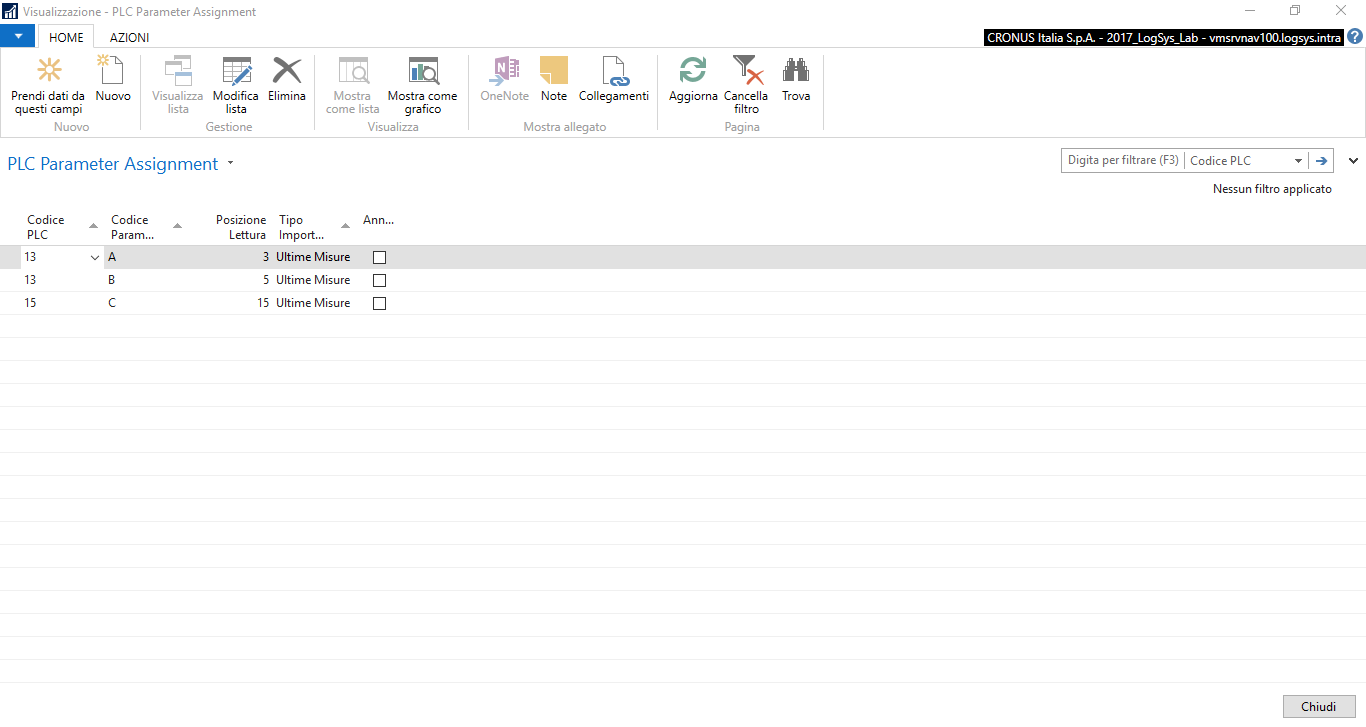
\includegraphics[width=0.8\textwidth]{PLC-Assigment-List.png}
	\caption*{Figura 18. La pagina PLC Parameter Assignment, dalla quale si impostano i valori da richiedere}
\end{figure}
\clearpage
\begin{figure}[H]
	\centering
	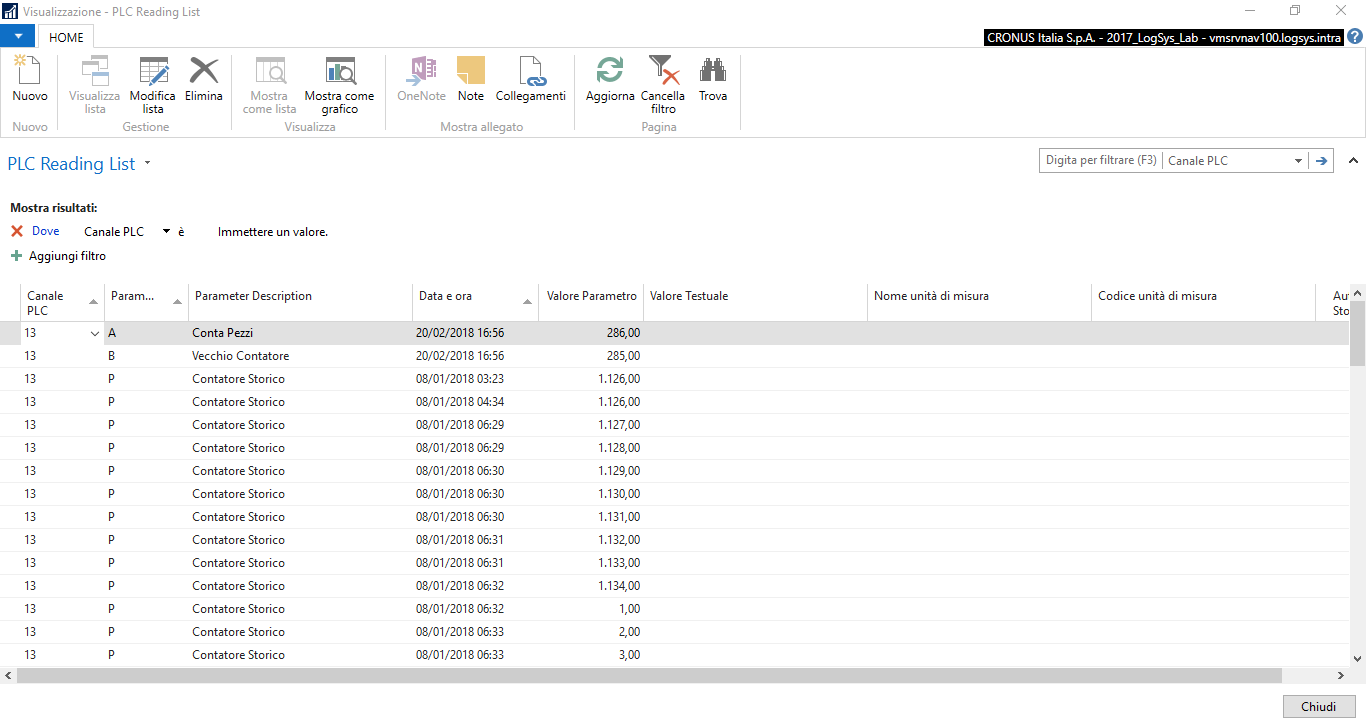
\includegraphics[width=0.8\textwidth]{PLC-Reading-List.png}
	\caption*{Figura 19. La pagina PLC Parameter Reading, dalla quale si visualizzano i valori richiesti}
\end{figure}
Per poter effettuare il servizio di sottoscrizione in NAV è stata generata la pagina SubscriptionPage, nella quale è presente la possibilità di scrivere le condizioni sulle quali si vogliono i dati (la clausola con cui si faranno chiamate in SQL), e si lancia una page action collegata alla codeunit con la quale si effettua il metodo di sottoscrizione in base alle informazioni riportate in input. Una volta ricevuta la risposta, in caso di esito affermativo, si prende il numero della sottoscrizione e si setta in tabella, impostando inoltre lo stato come attivo. Per cancellare una sottoscrizione è possibile dunque utilizzare la page action unsubscribe che partendo dal dato messo in tabella come ID Sottoscrizione lo invia alla piattaforma che procederà dunque a cancellare la sottoscrizione relativa. 
\clearpage
\section{Manualistica}
\subsection{Installazione e avvio della piattaforma}
La piattaforma si presenta come un jar eseguibile a cui è necessario fornire parametri di input. Un esempio per lanciare la piattaforma in locale è rappresentato in figura 18.
\begin{figure}[h]
			\centering
			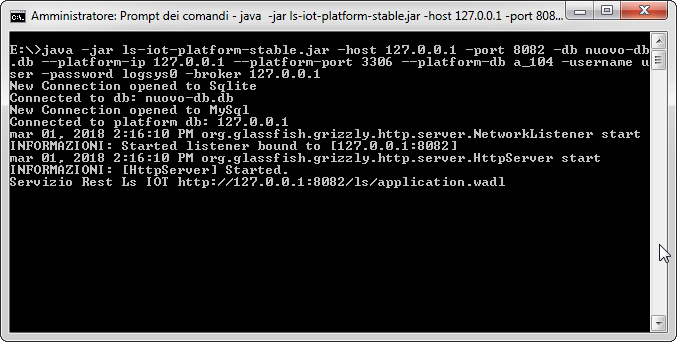
\includegraphics[width=0.8\textwidth]{lancio-piattaforma.png}
			\caption*{Figura 20. Avvio della piattaforma con parametri}
\end{figure}

I parametri sono:
{\fontfamily{pcr}\selectfont
	\lstinputlisting[breaklines]{launch-parameters.txt}
}
Il parametro host definisce l'indirizzo ip sul quale sarà in esecuzione la piattaforma, mentre il parametro port definisce la porta.
Il parametro db indica il path del database SQLite di amministrazione. Il comando opzionale ow è un'abbreviazione di overwrite e indica se il database già presente deve essere sovrascritto con un nuovo database di default nel momento in cui la piattaforma viene avviata. se ow è presente il database viene sovrascritto.
I tre parametri che contengono la parola platform indicano rispettivamente: indirizzo ip, porta e nome del database relativi al server in cui il database della backend è in esecuzione.
Username e password sono le credenziali con le quali avviene il collegamento al database della backend e sono opzionali. Infine broker indica l'indirizzo ip al quale il servizio activemq è in esecuzione. Se il parametro non è presente viene lanciato il broker embedded della piattaforma.
\clearpage
\subsection{Installazione servizio ActiveMQ esterno}
Per installare il servizio di ActiveMQ è necessario estrarre la cartella che si scarica dal sito ufficiale. Una volta ottenuta la cartella, deve essere lanciato il servizio di activemq da terminale tramite il comando 

$<path-to-activemq>/bin/activemq start$
\begin{figure}[h]
	\centering
	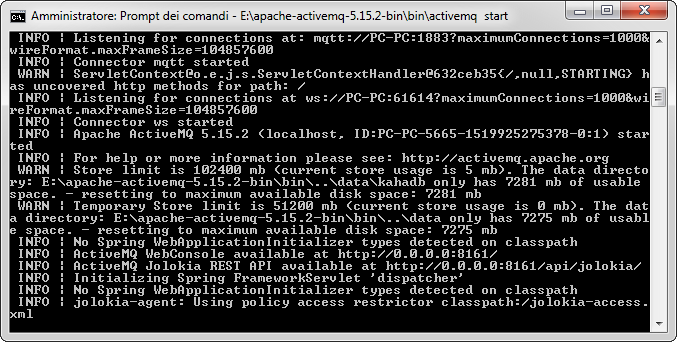
\includegraphics[width=0.8\textwidth]{activemq-in-esecuzione.png}
	\caption*{Figura 21. Istanza di activemq in esecuzione}
\end{figure}
\clearpage
\subsection{Interfaccia web Piattaforma}
La piattaforma ha una interfaccia web che permette di gestire le richieste. In figura 22 viene mostrata la pagina di richiesta che un utente visualizza nel momento in cui vuole abilitare la sua applicazione ad usare la piattaforma, mentre in figura 23 è rappresentata la pagina di gestione delle richieste che mostra cosa l'amministratore della piattaforma vede quando una nuova richiesta viene registrata.
\begin{figure}[h]
	\centering
	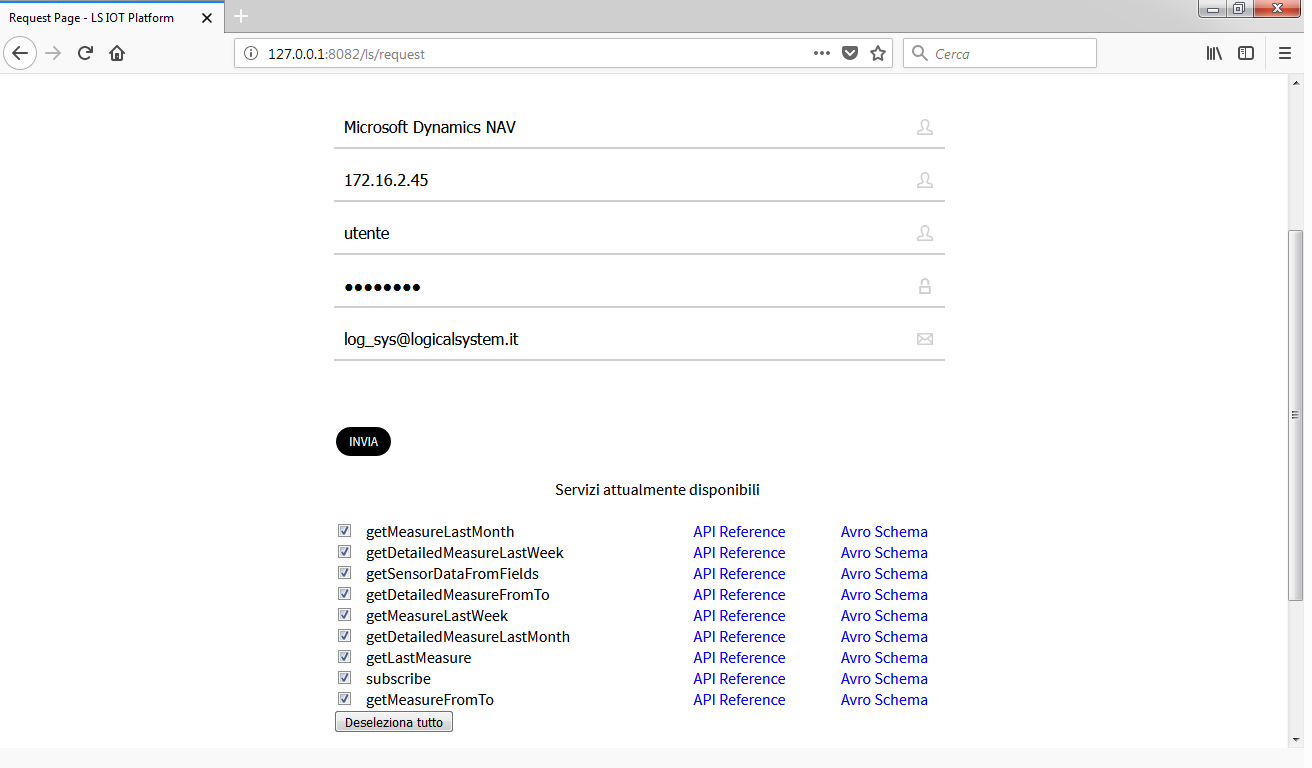
\includegraphics[width=0.75\textwidth]{pagina-di-richiesta.png}
	\caption*{Figura 22. Pagina di richiesta per utilizzare la piattaforma}
\end{figure}
\begin{figure}[h]
	\centering
	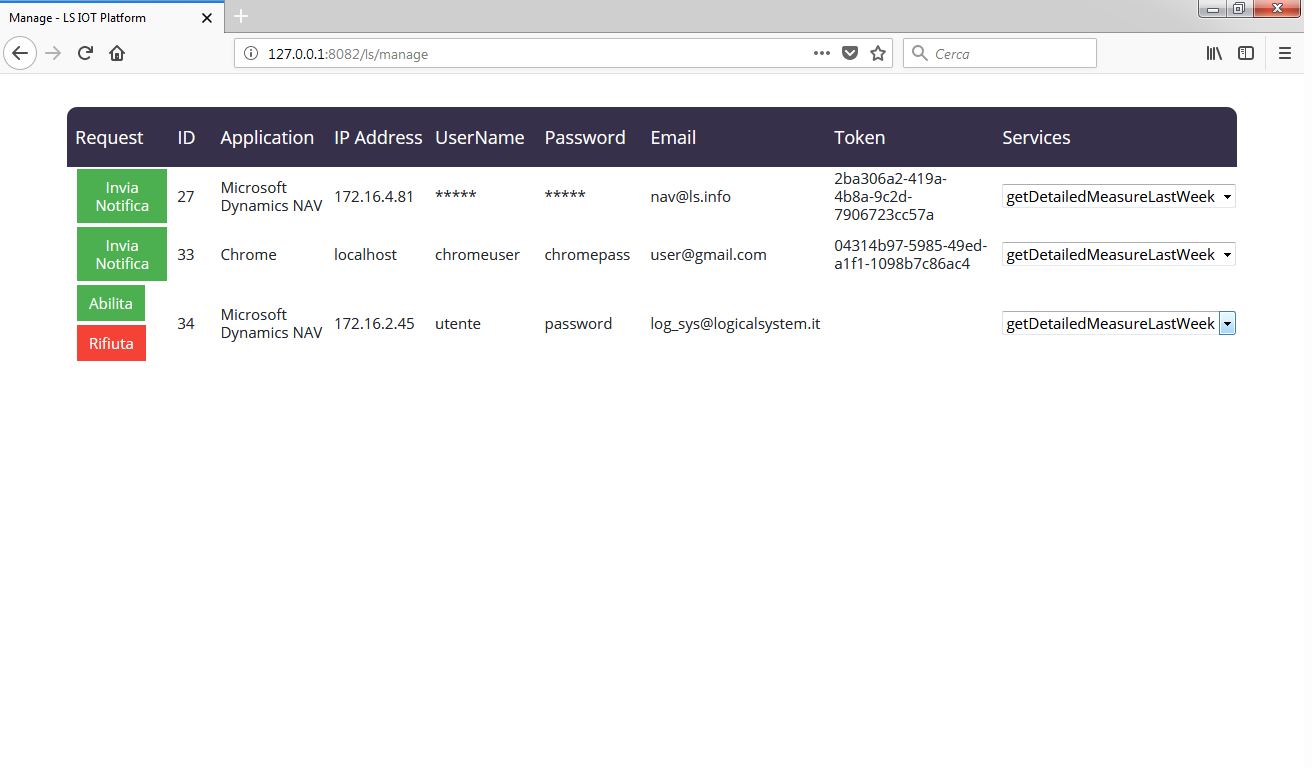
\includegraphics[width=0.75\textwidth]{gestione-delle-richieste.png}
	\caption*{Figura 23. Pagina di gestione delle richieste}
\end{figure}
\clearpage
\section{Possibili sviluppi futuri}
Come possibili sviluppi futuri sono attualmente previste la costruzione di un ontologia di dominio Logical System per la piattaforma LSIoT Platform tramite l'utilizzo di Protegè e SKOS (Simple Knowledge Organization System) e l'integrazione della piattaforma con il data streaming tramite l'utilizzo di Apache Flink per il monitoraggio degli eventi relativi alle misurazioni.
\end{document}